\documentclass[11pt,a4paper]{article}
\usepackage[margin=25mm]{geometry}
\usepackage[T1]{fontenc}
\usepackage[utf8]{inputenc}
\usepackage{lmodern}
\usepackage{graphicx,booktabs,tabularx,array,multirow,amsmath}
\usepackage{caption,placeins,enumitem}
\usepackage[most]{tcolorbox}
\usepackage[numbers,sort&compress]{natbib}
\usepackage[hidelinks]{hyperref}
\newcommand{\added}[2][]{#2}
\newcommand{\Description}[1]{}
\graphicspath{{figures/}{samples/figures/}}
\renewcommand{\thesection}{S\arabic{section}}
\renewcommand{\thetable}{S\arabic{table}}
\renewcommand{\thefigure}{S\arabic{figure}}
\setlength{\parskip}{4pt}
\setlength{\parindent}{0pt}
\setlength{\emergencystretch}{1em}
\title{Supplementary Material\\[6pt]\large Building Bayesian Networks in Software Engineering:\\A Checklist and Catalog of Methods for Expert-Based and Hybrid Models}
\author{Thiago Rique \and Emilia Mendes \and Mirko Perkusich \and Danyllo Albuquerque \and Kyller Gorg\^onio \and Angelo Perkusich}
\date{}
\begin{document}
\maketitle
This companion document provides mapping and agreement records, detailed method descriptions and application examples, and the activity-indexed catalog of retained software engineering studies. The checklist and catalog concern activities that directly specify, parameterize, or evaluate a Bayesian network (BN), assuming that a BN has been selected as the modeling approach. They are resources for consultation and documentation, not a prospectively evaluated construction methodology.

The complete study-selection, mapping, extraction, and assessment workbooks are available in the \href{https://github.com/mprkc/bn-construction-se}{supplementary repository}. P identifiers refer to the cross-domain methodology review; S1--S118 refer to the assessed SE studies; PS1--PS66 refer to studies retained for the catalog. The workbooks retain their original identifiers and terminology.

Abbreviations: SE, software engineering; DAG, directed acyclic graph; CPT, conditional probability table; EKEBN, Expert-Based Knowledge Engineering of Bayesian Networks.
\tableofcontents
\clearpage
\section{Mapping and Agreement Records}
\label{supp:mapping}
\subsection{Data Extraction and Mapping}

From the set of included articles, we extracted the data needed to address RQ1. For each proposed methodology, we identified the construction phases and the specific activities associated with each phase. The first author extracted the data and organized them in a spreadsheet. The second author reviewed the extracted data, and when disagreements arose, both researchers discussed the inconsistencies until they reached a consensus.

\added[id=A]{We initially employed an inductive coding approach to analyze and organize the phases and activities extracted from the selected methodologies. The analysis preserved the terminology and process organization reported in the original studies, allowing different activities and process structures to emerge from the literature. During this analysis, we observed substantial convergence between the emerging categories and the phases and activities defined in the EKEBN process proposed by Mendes~\cite{mendes2012using}.}

\added[id=A]{After observing this correspondence, and drawing on the authors' prior familiarity with EKEBN, we adopted its phases and activities as reference categories to facilitate subsequent deductive coding. The coding remained open to additional phases or activities within the checklist's scope. Unmatched activities were recorded under ``Others'' and examined in relation to that scope, rather than treating the reference categories as an exhaustive account of the modeling-project lifecycle. The treatment of these activities is reported with the mapping results below.}

\added[id=A]{The first three authors conducted the deductive mapping of the activities extracted from the methodologies (which we refer to as general activities) to the EKEBN process. This mapping consisted of two stages:}

\begin{itemize}
\item \textit{Mapping general activities to the EKEBN phases.} \added[id=A]{In this stage, we examined whether the activities identified in the analyzed methodologies could be organized according to the EKEBN phases or whether additional phases of the BN construction process emerged from the analysis.} All activities extracted from the methodologies were organized in a spreadsheet, along with the descriptions provided in the articles. Each researcher independently analyzed and classified the activities according to the EKEBN phases: structure building, parameter estimation, and model validation. Activities that did not correspond to any of these phases were assigned to the category ``Others.'' In cases of disagreement, the three researchers discussed the classifications until reaching a consensus. To assess inter-rater agreement, we calculated the Fleiss' Kappa coefficient ($\kappa$)~\cite{fleiss1971measuring}, whose value is presented in Table~\ref{tab:fleiss_kappa_stage1}. According to the interpretation proposed by Landis and Koch~\cite{landis1977measurement}, the researchers achieved an almost perfect level of agreement.

\item \textit{Mapping general activities to the EKEBN activities.} \added[id=A]{In this stage, we examined whether the activities retained within the checklist's scope could be organized according to the activities defined in EKEBN or whether additional BN construction activities emerged from the analysis. The input consisted of the activities grouped by construction phase after the first-stage mapping and scope exclusions described below.} Each researcher analyzed these activities individually and classified them according to the activities defined for each EKEBN phase. Activities related to structure building were classified as ``identification of nodes/variables,'' ``identification of node values/states,'' ``identification of relationships,'' or ``structure evaluation.'' Activities related to parameter estimation were classified according to categories associated with ``CPT construction'' and ``CPT evaluation.'' Finally, activities related to model validation were classified as ``expert-based validation'' or ``data-driven validation.'' \added[id=A]{An ``Others'' category was again available for unmatched activities, but none of the retained activities required it in this second stage.} As in the previous stage, some activities generated classification disagreements. In such cases, the three researchers discussed the divergences until reaching a consensus. The Fleiss' Kappa coefficient ($\kappa$) was also calculated in this stage to assess inter-rater agreement. The values of the coefficient for activity mapping within each phase, along with their interpretation, are presented in Table~\ref{tab:fleiss_kappa_stage2}.
\end{itemize}

\begin{table}[t]
\caption{Fleiss' $\kappa$ coefficient for inter-rater agreement (first stage of the analysis)}
\label{tab:fleiss_kappa_stage1}
\centering
\small
\renewcommand{\arraystretch}{1.15}
\setlength{\tabcolsep}{10pt}

\begin{tabular}{lc}
\toprule
\textbf{$\kappa$ value} & \textbf{Level of agreement} \\
\midrule
0.93 & Almost perfect \\
\bottomrule
\end{tabular}
\end{table}

\begin{table}[t]
\caption{Fleiss' $\kappa$ coefficients for inter-rater agreement by phase (second stage of the analysis)}
\label{tab:fleiss_kappa_stage2}
\centering
\small
\renewcommand{\arraystretch}{1.15}
\setlength{\tabcolsep}{10pt}

\begin{tabular}{lcc}
\toprule
\textbf{Phase} & \textbf{$\kappa$ value} & \textbf{Level of agreement} \\
\midrule
Structure building     & 0.72 & Substantial \\
Parameter estimation  & 1.00 & Almost perfect \\
Model validation      & 0.74 & Substantial \\
\bottomrule
\end{tabular}
\end{table}

\subsection{Mapping Results}

Next, we present the results and analysis of the systematic review. The list of selected articles and the mapping results are available in the supplementary ~\cite{rique2026supplementary}.



To address RQ1, we extracted the phases and activities described in the BN construction process from each methodological article. The extraction followed a descriptive approach that preserved the terminology used by the studies' authors, respecting the original ways in which each paper used a methodology to structure the BN processes. The results revealed substantial heterogeneity in how the methodologies organize the construction process, showing both common phases and activities and elements that capture aspects unique to each proposed approach. Although different methodologies refer to similar activities using distinct terminology (e.g., ``identify variables'' vs. ``identify key factors''), we retained the descriptions exactly as they appear in the original articles. This decision preserves the integrity of each methodology's contribution and enables a more faithful analysis of convergences and divergences in later stages.

The extraction produced a spreadsheet (see~\cite{rique2026supplementary}) containing all phases and activities reported in the analyzed articles. For example, P13 proposed the following phases: ``Identify the objective,'' ``Develop the network structure,'' ``Formalize the model structure,'' ``Quantify the model,'' ``Interrogate the BN model,'' ``Validate the BN model,'' and ``Communicate BN results.'' Within the ``Identify the objective'' phase, the methodology included the activity ``Identify one top-level node.'' Within ``Develop the network structure,'' the proposed activities were ``Identify key factors,'' ``Identify remaining factors,'' ``Identify node states,'' and ``Identify relationships.'' Another example of an article that organized the construction process differently is P17, which defined the following phases: ``Explore problem,'' ``Variables,'' ``Structure,'' ``Parameters,'' ``Explore network,'' and ``Report.'' Within ``Variables,'' the proposed activities were ``Specify BN variables'' and ``Specify discrete states of BN variables.'' Within the ``Structure'' phase, the ``Specify relationships'' activity was included.

The resulting spreadsheet provides an overview of the activities considered across methodologies and serves as the basis for mapping these activities to the EKEBN process. During the mapping process, the need to split certain activities for greater clarity emerged from the researchers' individual analyses and was subsequently discussed and consensually validated during the joint meetings. For example, the activity ``Add, delete, or modify nodes and directed links'' in P16 was separated into ``Add, delete, or modify nodes'' and ``Add, delete, or modify directed links.'' The mapping process aimed to eliminate redundancies, identify gaps, and consolidate a reference process for constructing expert-based or hybrid BN models. 

\added[id=A]{The first deductive mapping stage assigned the general activities extracted from each article to an EKEBN phase or to ``Others.''} Table~\ref{tab:map_stage1_examples} presents examples of this mapping (the complete mapping is documented in the supplementary material~\cite{rique2026supplementary}).

\begin{table}[t]
\caption{Examples of activities mapped to EKEBN phases in the first stage of the analysis}
\label{tab:map_stage1_examples}
\centering
\small
\renewcommand{\arraystretch}{1.2}
\setlength{\tabcolsep}{8pt}

\begin{tabularx}{\linewidth}{>{\raggedright\arraybackslash}X
                              >{\centering\arraybackslash}p{1.2cm}
                              >{\raggedright\arraybackslash}p{2.5cm}}
\toprule
\textbf{Activity} & \textbf{Paper} & \textbf{Phase} \\
\midrule
Determine model objective & P1 & Others \\
Identify the initial set of nodes & P1 & Structure building \\
Expert review of predictions & P2 & Model validation \\
Eliminate cycles & P4 & Structure building \\
Derivation of the conditional probabilities associated with the variables in the map & P10 & Parameter estimation \\
Populate conditional probability tables (CPTs) & P16 & Parameter estimation \\
\bottomrule
\end{tabularx}
\end{table}

\begin{table}[t]
\caption{Activities classified as ``Others'' in the first stage of the analysis}
\label{tab:map_stage1_others}
\centering
\small
\renewcommand{\arraystretch}{1.2}
\setlength{\tabcolsep}{8pt}

\begin{tabularx}{0.70\linewidth}{>{\raggedright\arraybackslash}X
                              >{\centering\arraybackslash}p{1.2cm}}
\toprule
\textbf{Activity} & \textbf{Paper} \\
\midrule
Determine model objective & P1 \\
Perform decision analysis & P1 \\
Validate objective & P13 \\
Create the modes of results communication & P13 \\
Identify the hypotheses suggested by the problem/questions & P17 \\
Identify the items of evidence most pertinent to those hypotheses & P17 \\
Develop report & P17 \\
Determine quantification approach & P25 \\
Collate relevant information & P25 \\
Determine assessment baseline & P25 \\
Perform validation of the objective & P25 \\
Identifying the stakeholders & P29 \\
Defining the question the BN is supposed to answer & P29 \\
Identifying suitable data and information to build the model & P29 \\
Selecting experts & P29 \\
Selecting appropriate tools & P29 \\
\bottomrule
\end{tabularx}
\end{table}

\added[id=A]{The first-stage mapping identified activities that did not correspond directly to the EKEBN phases. These activities were recorded as ``Others'' (Table~\ref{tab:map_stage1_others}) and were not retained in the checklist. The checklist's scope concerns activities that directly specify, parameterize, or evaluate the BN itself, assuming that a BN has been selected as the modeling approach. It does not cover the entire modeling-project lifecycle. The exclusions concern the following types of activities:}

\begin{itemize}
\item \added[id=A]{Project-level preparation, context definition, and approach selection. These include defining or checking project objectives, identifying stakeholders and available information sources, and selecting experts, tools, or an overall modeling approach. Such activities support the modeling project but are outside the checklist's focus on constructing and validating the BN.}

\item \added[id=A]{Model use and communication. These include establishing a baseline for decision analyses, using the model to support decisions, communicating results, and preparing reports. They concern the application and communication of the model rather than its construction or validation and were not included as checklist activities.}
\end{itemize}

\added[id=A]{This is a functional scope boundary, not a requirement that activities occur in a fixed temporal order or be exclusive to BNs. Identifying variables that become BN nodes and validating the BN remain within scope even though analogous activities occur in other modeling approaches. Conversely, excluding project-level preparation or model-use activities does not imply that they are unnecessary for a successful modeling project.}

\added[id=A]{P25~\cite{chakraborty2015multifaceted} illustrates the distinction. We interpreted ``Determine quantification approach'' as selecting and motivating the overall quantitative modeling approach; the corresponding passage discusses alternatives such as regression and factor analysis before introducing BNs. It was classified as ``Others.'' The separate activity ``Quantify model,'' which describes estimating BN probability distributions, was retained under parameter estimation and subsequently mapped to CPT construction. Thus, the classification distinguishes approach selection from parameter estimation, even though P25 places both activities within its Quantification stage.}

\added[id=A]{After these scope exclusions, the retained activities were organized into the three EKEBN phases. These phase-level groups provided the input for the second mapping stage.}

\added[id=A]{In the second mapping stage, all retained activities could be accommodated by the EKEBN activities, and none required the ``Others'' category. Table~\ref{tab:map_stage2_examples} presents examples per phase (the complete mapping is available in the supplementary material~\cite{rique2026supplementary}). This finding supports the use of EKEBN as an organizing framework for the activities retained in this synthesis. It does not independently establish EKEBN's completeness, because the finding is conditional on the reviewed corpus and the checklist's scope.}

\begin{table}[t]
\caption{Examples of activities mapped to EKEBN activities in the second stage of the analysis}
\label{tab:map_stage2_examples}
\centering
\small
\renewcommand{\arraystretch}{1.2}
\setlength{\tabcolsep}{8pt}

\begin{tabularx}{\linewidth}{>{\raggedright\arraybackslash}X
                              >{\centering\arraybackslash}p{1.2cm}
                              >{\raggedright\arraybackslash}p{3.2cm}}
\toprule
\textbf{Activity} & \textbf{Paper} & \textbf{EKEBN Activity} \\
\midrule

\multicolumn{3}{l}{\textbf{Structure building}} \\
Introduce synthetic variables & P1 & Identification of nodes/variables \\
Manage mutual exclusivity & P1 & Identification of node values/states \\
Build initial causal graph & P4 & Identification of relationships \\
Revise causal graph with experts & P4 & Structure evaluation \\

\addlinespace[6pt]
\multicolumn{3}{l}{\textbf{Parameter estimation}} \\
Learning parameters with insufficient data & P7 & CPT construction \\
Populate conditional probability tables (CPTs) & P16 & CPT construction \\
Evaluate CPTs & P16 & CPT evaluation \\

\addlinespace[6pt]
\multicolumn{3}{l}{\textbf{Model validation}} \\
Performance evaluation (in terms of discrimination, calibration, and accuracy) & P7 & Data-driven validation \\
Validate results with experts & P13 & Expert-based validation \\

\bottomrule
\end{tabularx}
\end{table}

\begin{tcolorbox}[
    colback=gray!5,
    colframe=black,
    boxrule=0.5pt,
    arc=2pt,
    left=6pt,
    right=6pt,
    top=6pt,
    bottom=6pt
]
\textbf{RQ1 --- What are the fundamental activities involved in constructing expert-based or hybrid BNs?}

The analysis revealed significant heterogeneity in how methodologies describe and group BN construction activities. Some approaches focus narrowly on activities directly related to network construction, while others also include more general modeling steps, such as defining objectives, scope, and context. \added[id=A]{Within the scope retained for the checklist, the activities were organized into:}
(i) structure building (including identification of variables, states, relationships, and structure evaluation),
(ii) parameter estimation (including CPT construction and evaluation), and
(iii) model validation (expert-based or data-driven).

\added[id=A]{EKEBN accommodated the retained activities across the analyzed methodologies and provided the organizing framework for the checklist. This coverage concerns the construction and validation activities included in the synthesis, rather than the entire modeling-project lifecycle.}
\end{tcolorbox}

\clearpage
\section{Methods and Detailed Application Examples}
\label{supp:methods}

\added[id=A]{This section presents methods extracted from the studies that met the catalog inclusion threshold. For each construction phase, the methods are described alongside examples of their reported application. Studies often combine methods within an activity; their inclusion here records their use rather than establishing their suitability for every modeling context.}

\added[id=A]{The scope of this analysis extends substantially beyond our previous mapping study~\cite{rique2025constructing}, which focused specifically on methods for constructing the structure of expert-based BNs in SE. The present study considers both expert-based and hybrid BNs and organizes the identified methods according to the complete set of construction activities defined in the checklist, encompassing structure building, parameter estimation, and model validation. Methods previously identified in~\cite{rique2025constructing} are intentionally retained and integrated with the additional evidence to provide a self-contained catalog covering the complete BN construction process.}

\subsection{Structure Building}

The methods identified for performing the four activities related to the \textbf{structure building} phase are described next. We observed that during this construction phase, the application domain (i.e., SE) strongly influences the choice of modeling methods, particularly the types of reasoning employed.

\vspace*{0.5\baselineskip}

\textbf{Methods for identifying variables and relationships.} The activities of identifying variables and relationships are closely intertwined during structure building, often occurring in parallel. Therefore, they are addressed jointly to avoid redundant method descriptions. Extending the classification scheme proposed by Rique et al.~\cite{rique2025constructing}, we inductively classified the identified methods into three dimensions: knowledge acquisition, reasoning mechanisms, and automatic construction.

The \textbf{knowledge acquisition} dimension comprises methods for collecting and analyzing data related to domain experts' experience and viewpoints, as well as findings from the literature on SE aspects relevant to the construction of a BN structure. It also includes the analysis of software data and artifacts. Table~\ref{tab:knowledge-acquisition-methods} lists the methods within the knowledge acquisition dimension, which are described below:

\begin{table}[t]
\caption{Knowledge acquisition methods used for the identification of variables (Activity 1.1) and relationships (Activity 1.3)}
\label{tab:knowledge-acquisition-methods}
\centering
\small
\setlength{\tabcolsep}{6pt}
\renewcommand{\arraystretch}{1.2}

\begin{tabularx}{\linewidth}{>{\raggedright\arraybackslash}p{0.26\linewidth}
                              >{\raggedright\arraybackslash}X
                              >{\raggedright\arraybackslash}X}
\toprule
\textbf{Method} & \textbf{1.1: Variables} & \textbf{1.3: Relationships} \\
\midrule
Interviews
& S1, S3, S5, S24, S26, S67, S74, S81, S107, S111
& S1, S8, S24, S26, S74, S81, S107 \\
Focus groups
& S3--S6, S27, S75, S81, S114
& S3--S6, S27, S75, S81 \\
Survey with practitioners
& S103, S104, S114
& S67, S103, S104, S107, S108, S111 \\
Literature review
& S2, S4, S6--S8, S10, S14, S20, S21, S25, S27, S29, S33, S35--S38, S44, S52, S54, S58, S67, S68, S72, S73, S75--S78, S80, S85, S87, S92--S94, S96, S101, S104, S107, S108, S111, S113
& S2, S4, S6, S7, S20, S21, S25, S27, S29, S33, S35--S38, S40, S44, S52, S58, S68, S72, S73, S75--S78, S80, S85, S87, S92--S94, S96, S101, S104 \\
Selection of variables from a dataset
& S4, S6, S38, S40
& --- \\
Delphi method
& S7
& S7 \\
Abstraction sheets
& S1
& S1 \\
Grounded theory
& S3, S5, S74, S103, S104
& S74, S103, S104 \\
Statistical analysis
& ---
& S20, S54 \\
Software analysis
& S59
& S59 \\
\bottomrule
\end{tabularx}
\end{table}

\textit{Interviews.} Interviews are a widely used method in SE for eliciting expert knowledge. This method relies on individuals with experience across various aspects of software development. After interviews are conducted, the collected data are typically analyzed to extract meaningful insights and patterns. Such analysis can help identify common themes, trends, and valuable information shared by experts. The analysis of interview data aims to identify relevant variables and relationships that delineate the DAG of the BN modeling the SE problem under consideration. Some studies used interviews with a rigorous, systematic approach, analyzing the collected data with well-established coding techniques from the qualitative research literature (e.g., S3 and S5). Another example is S8, in which the authors interviewed a domain expert to derive relationships among factors identified in an SLR. As a method for eliciting expert knowledge that underpins model construction, it is essential that the data from the interview process be appropriately analyzed.

\textit{Focus groups.} Using focus groups to elicit expert knowledge involves bringing together a group of subject-matter experts to collaboratively discuss specific topics or issues related to software development. As in the study by Rique et al.~\cite{rique2025constructing}, this study considers workshops, expert panels, and brainstorming sessions as focus groups, given their shared emphasis on group interaction and discussion. The studies applied focus groups mainly in two ways: to elicit and validate factors and relationships. For example, S3 demonstrated the versatility of focus groups in both applications. The authors used focus groups to complement the knowledge elicitation process by discussing and reaching consensus on a set of value factors initially identified through interviews. Also, they validated the BN structure through focus groups with experts. Another example is S114, in which the authors consulted experts to identify relevant model factors through a questionnaire and brainstorming sessions.

\textit{Survey with practitioners.} When it comes to eliciting expert knowledge to construct BN structures, surveys serve as a valuable method for capturing practitioners' opinions and experiences in a structured and quantifiable manner. Survey questions are carefully designed to address specific aspects of interest, such as factors influencing decision-making or dependencies among different variables. We observed that surveys can be used across different activities. Regarding the identification of variables and relationships, the authors of S104 constructed a BN across multiple companies by analyzing and coding textual data from a survey containing practitioners' responses about \added[id=A]{what they perceived as the main causes and effects of requirements engineering problems}. The authors of S67 \added[id=A]{collected questionnaire data to inform proposed cause-effect relationships among factors} extracted from a literature review and interviews with domain experts.

\textit{Literature review.} Another common way of constructing BN structures is using the literature review method. Software researchers and practitioners rely on evidence from existing literature to reason about variables and relationships to be incorporated into their models. The notion of literature review considered here encompasses different approaches, as described in Rique et al.~\cite{rique2025constructing}. It may refer to searching for insights or structured knowledge in the scientific literature (e.g., S25), guidelines (e.g., S7), reports and standards (e.g., S101), or a more rigorous approach involving an SLR (e.g., S72). The authors of S7 constructed BNs to assess Scrum-based software development methods and explored the Scrum Guide to build their structures. For model construction in S101, the IEEE Standard 1012 (V\&V) was used primarily to identify attributes and their associated activities, along with several other reports and standards, including IEC 60880, DO-178C, NUREG/CR-6101, and BTP-14. In contrast, the authors of S72 conducted an SLR that identified more than 50 attributes across different categories influencing user story estimation. Thus, notable differences can be observed in how this method is applied and reported across studies.

\textit{Selection of variables from a dataset.} The initial structure of a BN can be outlined based on the selection of variables from existing datasets relevant to the SE problem being addressed. Drawing on their prior experience in building BN models, the authors of S4 used the variables from the Tukutuku project as a starting point to identify the factors domain experts consider when estimating effort in Web applications. After the knowledge engineer outlined and explained the variables, the domain experts suggested removing irrelevant variables and adding new ones. Another example is S38, in which the authors used variables from the COCOMO II model and existing studies to propose a causal model for software effort prediction. Similarly, S40 constructed a BN for productivity estimation based on the cost factors of COCOMO 81.

\textit{Delphi method.} Researchers can use the Delphi method to make the process of eliciting expert knowledge more systematic and less biased when compared to approaches such as focus groups. The authors of S7 decomposed the nodes of their BN into initial elements representing the main software process factors, which were then presented to the experts. Subsequently, the authors applied the Delphi method to refine these sets of elements through individual rounds of discussion, thereby influencing the model's variables and relationships.

\textit{Abstraction sheets.} S1 used abstraction sheets as a support tool for interviews within the Goal-Question-Metric (GQM) process, serving to identify the variables and relationships of the BN. Through their quadrants, relevant questions and metrics corresponding to the quality focus --- affected by variation factors given the defined goal --- were extracted. In this way, abstraction sheets provided a structured mechanism for translating expert knowledge into model elements and dependencies.

\textit{Grounded Theory.} Grounded Theory (GT) is a qualitative research methodology often used to develop theories through the systematic analysis of data without preconceived notions or predefined structures~\cite{urquhart2022grounded}. Researchers collect data using different methods, such as interviews, observations, and open-ended surveys. In the context of SE, both full GT studies aimed at theory generation and applications of GT principles for qualitative data analysis can be found. The results of both approaches have been used to construct BNs' DAGs. For example, the authors of S74 built the core fragment of their BN model using results from a full GT study that interviewed twenty-five practitioners from ten organizations. The authors of S103 relied on survey data that were manually coded following GT principles. Thus, GT plays an important role in the construction of expert-based BN structures, as it helps identify relevant variables represented by the key concepts and categories that emerge from qualitative data. The relationships among these variables are explored and defined based on a grounded understanding of the SE phenomenon under study. By contrast, S5 collected interview data that were analyzed using GT principles. The resulting codes represented factors to be used as part of the DAG construction phase. The analysis results were then used in a focus group, where experts suggested removing irrelevant factors or adding new ones to the model.

\textit{Statistical analysis.} \added[id=A]{Domain experts may use statistical analyses to identify associations among variables and inform the BN structure.} Due to data issues, a sensible strategy is to build the model incorporating expert knowledge and judgment about the statistical analysis results, instead of automatically generating the model from the data. \added[id=A]{In S20, chi-plot independence tests informed the relationships in the hybrid model; such tests do not by themselves establish cause-effect relationships.} To explore the relationship between multiple project metrics and different fault categories, the authors of S54 conducted a bivariate correlation analysis (Spearman correlation). 

\textit{Software analysis.} Experts may reflect on the results of software analysis, such as static and/or dynamic analyses, to identify variables and relationships. For example, S59 employed static analysis to extract information about software elements' dependencies, which served as the basis for constructing the graphical structure of the models.

The \textbf{reasoning mechanisms} dimension comprises methods that support domain experts in establishing the types of reasoning appropriate to the relationships they intend to use to model the DAG. In addition, it involves the use of techniques to guide experts' reasoning towards specific SE aspects on which they wish to focus, or to assist in the application of concepts inherent to BN modeling. Table~\ref{tab:reasoning-mechanisms-methods} presents the methods within the reasoning mechanisms dimension, which are described next.

\begin{table}[t]
\caption{Reasoning mechanisms used for the identification of variables (Activity 1.1) and relationships (Activity 1.3)}
\label{tab:reasoning-mechanisms-methods}
\centering
\small
\setlength{\tabcolsep}{6pt}
\renewcommand{\arraystretch}{1.2}

\begin{tabularx}{\linewidth}{>{\raggedright\arraybackslash}p{0.32\linewidth}
                              >{\raggedright\arraybackslash}X
                              >{\raggedright\arraybackslash}X}
\toprule
\textbf{Method} & \textbf{1.1: Variables} & \textbf{1.3: Relationships} \\
\midrule
Idioms
& S7, S20, S48, S81, S85, S93
& S7, S20, S48, S81, S85, S93 \\
Divorcing
& ---
& S3--S6, S85, S87 \\
D-separation
& ---
& S4, S12, S94 \\
Life cycle model (SDLC)
& S14, S23, S27--S29, S31, S94, S95, S101
& S14, S23, S27--S29, S31, S94, S95, S101 \\
Risk-centric modeling
& S67, S74, S78, S93, S104, S107, S108
& S67, S74, S78, S93, S104, S107, S108 \\
GQM paradigm
& S1, S10, S12, S18, S81, S85
& S1, S10, S12, S18, S81, S85 \\
Top-down approach
& S7, S8, S73
& S7, S8, S73 \\
Quality model
& S53, S75, S88
& S53, S75, S88 \\
Value model
& S3
& S3 \\
Argumentation model
& S43
& S43 \\
\bottomrule
\end{tabularx}
\end{table}

\textit{Idioms.} The use of idioms for constructing BN structures is based on the concept of ``building blocks'' that function as solution patterns. Idioms describe distinct BN fragments that embody generic forms of uncertain reasoning employed by experts during model construction and can be integrated to form more comprehensive BNs~\cite{neil2000building}. As such, they are closely related to the identification of variables and relationships in the models. Only a few studies explicitly mentioned the use of idioms to construct BNs. Rique et al.~\cite{rique2025constructing} identified the types of idioms applied in each study of their mapping and found that the most commonly used in the SE domain are the cause-consequence idiom (e.g., S20, S48, and S81), the definitional/synthesis idiom (e.g., S7 and S20), and the measurement idiom (e.g., S48 and S81).

\textit{Divorcing.} Technique used in BN construction whereby additional variables are introduced into the model to reduce the size of probability distributions and/or keep the network structure simpler. For example, in S4, the knowledge engineer used divorcing as an optimization procedure when she assumed that the final network structure had already been obtained, but still needed to reduce the number of probabilities to be elicited or learned. Another example is S85, which presents a BN-based approach for assessing the quality of Web applications. The authors collected and refined quality characteristics, constructed the model structure based on them, and derived the model parameters. However, because a node with 9 parents existed within a subnetwork of the model, it was necessary to restructure this subnetwork to avoid a combinatorial explosion during CPT elicitation. This was achieved by creating synthetic nodes to simplify the BN fragment. Therefore, divorcing is related to the structuring of relationships among variables, as it modifies how dependencies are modeled to simplify the network.

\added[id=A]{\textit{D-separation.} D-separation identifies conditional independences implied by a BN's graph. Examining these independences helps modelers assess whether the structure is consistent with their domain assumptions about how evidence should inform beliefs about other variables~\cite{mendes2012applying}. This is a check of the model's probabilistic structure, not a test establishing causality. Examples of studies that mention this approach include S4, S12, and S94.}

\textit{Life cycle model.} A common reasoning framework for constructing BNs is using the structured phases of the Software Development Life Cycle (SDLC) as a reference. Its application supports the identification of variables and relationships. This framework models the risks, tasks, and outcomes associated with each phase of software development, from requirements elicitation and design to implementation and maintenance. BNs constructed using this framework reflect the sequential or iterative nature of software projects and aim to manage uncertainty and risk at each life cycle phase. For example, S27 modeled the waterfall life cycle to predict software defects early in the development process. The cause-consequence idiom was used to model the relationships among key life cycle factors, while the definitional/synthesis idiom was used to organize the BN into subnetworks for key SDLC processes, such as ``specification and documentation,'' ``design and development,'' and ``testing and rework.'' In addition, indicator nodes were used to assess the quality of different processes; for instance, for ``testing process quality,'' the suggested indicators included ``quality of documented test cases,'' ``testing process well defined,'' and ``testing staff experience.''

\textit{Risk-centric modeling.} Some studies adopted a risk-centric modeling framework as the basis for constructing the DAG, delineating its variables and relationships. This framework focuses on the direct relationships and interactions among risk elements, such as threats, vulnerabilities, controls, and impacts. BNs built using this framework aim to capture and quantify the probabilistic dependencies among these risk factors, \added[id=A]{supporting predictions of risk conditional on specified technologies and mitigation strategies}. For example, S74 constructed a BN to predict risks in software projects given the technologies used (i.e., risk drivers) and the mitigation strategies employed. For this purpose, the definitional/synthesis idiom was applied to organize a hierarchical risk structure (e.g., ``integration risks'' and ``environment risks'' as parent nodes of ``infrastructure risks''). In addition, the cause-consequence idiom was employed to \added[id=A]{represent hypothesized cause-effect relationships between technologies} (e.g., ``JWT'' and ``Keystore'') and mitigation strategies (e.g., ``offline data persistence'') and risk factors (e.g., ``security risks'').

\textit{GQM paradigm.} The Goal-Question-Metric (GQM) paradigm guides experts' reasoning when conceptualizing the BN structure through a goal-oriented approach, defining the model's variables and relationships. 
For example, S1 used the GQM paradigm with experts to select software metrics for its model by employing indicator nodes. Another example is S18. Because the problem definition and the main key performance indicators (KPIs) are derived from the model's initial goal, the authors applied the GQM paradigm to identify relevant KPIs (i.e., definitional/synthesis idiom) and their relationships (i.e., cause-consequence idiom) to construct the causal structure of the proposed BN. S85 presented an approach for modeling the quality of Web applications using BNs. The authors gathered quality criteria specific to Web applications from existing work and refined them by applying the GQM paradigm, which reduced subjectivity and improved rigor through structured reasoning when confirming the selection of subcriteria and identifying metrics for the model. Thus, the authors of S85 used the criteria collected and refined through the GQM process to construct the graphical structure of the model, as they represented the BN nodes.

\textit{Top-down approach.} The variables and relationships of a BN structure can be identified by employing a top-down approach (e.g., S7 and S8). In both cases, the authors identified a top-level target node (i.e., process quality in S7 and teamwork quality in S8) and decomposed it into factors observed by the models' users, in a manner similar to the GQM paradigm, where goals are decomposed into questions and subsequently into metrics. The application of this approach led to the use of the definitional/synthesis and cause-consequence idioms. For example, in S7, the definitional/synthesis idiom was applied to decompose a node representing the personal characteristics of the Product Owner, a Scrum role, into multiple nodes (e.g., communicator and negotiator). Also, the cause-consequence idiom was employed to \added[id=A]{represent hypothesized effects of the Product Owner on the Product Backlog's quality and of the Product Backlog's quality on the effectiveness of Sprint Planning events}.

\textit{Quality model.} Quality attributes such as reliability, usability, performance, and maintainability are used as primary nodes in a BN. For example, S75 adopted this approach to identify the model's variables and relationships. The authors focused on estimating strategic software indicators (e.g., ``product quality'') by decomposing them into quality factors (e.g., ``code quality,'' ``testing status,'' and ``software stability'') that were, in turn, decomposed into measures using the definitional/synthesis idiom. 

\textit{Value model.} S3 constructed BNs by modeling the various factors and their interdependencies that contribute to the overall value delivered by a software system or project. The authors used the cause-consequence idiom to \added[id=A]{represent hypothesized effects of value factors on the delivered value}. A common scenario involved a BN including multiple value dimensions (i.e., nodes), such as ``market competitiveness,'' ``customer satisfaction,'' ``business value,'' and ``cost efficiency.'' As a result, these value dimensions were aggregated into an ``overall value'' node using the definitional/synthesis idiom.

\textit{Argumentation model.} S43 applied an argumentation model to represent the logical structure of composite arguments --- referred to as multilegged arguments --- that support dependability claims in software-based systems, particularly in safety-critical contexts. Each ``leg'' of the argument represents a distinct line of reasoning (e.g., statistical testing or formal verification), along with its associated evidence, assumptions, and uncertainties. The BN models the probabilistic relationships among these different argumentative lines, the supporting elements (such as the correctness of the specification or the test oracle), and the degree of confidence assigned to the main claim (e.g., that the system's probability of failure is below a certain threshold). The model enables the formal combination of different sources of evidence and allows exploration of how dependencies or correlations among elements affect the overall confidence in the argument.

The \textbf{automatic construction} dimension considers methods that automatically build the DAG from data using structure learning algorithms. It is important to note that, since our study does not focus on purely data-driven models, the model structures resulting from the automatic construction process \added[id=A]{involved input from domain experts}. \added[id=A]{A structure learned from observational data is not automatically a causal model; causal interpretation requires additional assumptions about the data-generating process and the variables represented~\cite{heckerman1995a}.} The methods within the automatic construction dimension are presented in Table~\ref{tab:metodos_construcao_automatica} and described next.

\begin{table}[t]
\caption{Automatic construction methods used for the identification of variables (Activity 1.1) and relationships (Activity 1.3)}
\label{tab:metodos_construcao_automatica}
\centering
\small
\setlength{\tabcolsep}{6pt}
\renewcommand{\arraystretch}{1.2}

\begin{tabularx}{\linewidth}{>{\raggedright\arraybackslash}p{0.34\linewidth}
                              >{\raggedright\arraybackslash}X
                              >{\raggedright\arraybackslash}X}
\toprule
\textbf{Method} & \textbf{1.1: Variables} & \textbf{1.3: Relationships} \\
\midrule
K2 algorithm
& S110
& S110, S114 \\
NPC algorithm
& S113
& S113 \\
Cheng's algorithm
& ---
& S107, S108 \\
V-structure discovery algorithm
& ---
& S108 \\
Learning from data using an automated tool
& S116, S118
& S3, S111, S116, S118 \\
\bottomrule
\end{tabularx}
\end{table}

\textit{K2 algorithm.} One of the earliest algorithms developed for BN structure learning is K2, proposed by Cooper and Herskovits~\cite{cooper1992bayesian} in 1992. This algorithm assumes that a predefined ordering among the nodes is available. Following this ordering, K2 iterates through the list of variables and greedily adds connections (edges) from candidate parent nodes that precede the current node in the order, aiming to maximize the K2 score~\cite{kitson2023survey}. In S110, the authors applied the K2 algorithm to a dataset. Although the resulting structure suggested interesting relationships among the variables, intuition-based refinement was required, during which some nodes were included, and others were excluded. In S114, the authors consulted experts using a questionnaire and brainstorming sessions to identify factors that may influence the software schedule at each development phase. When constructing the structure automatically, data imprecision may cause some relationships to be omitted or may link nodes that are in fact unrelated. For this reason, the authors defined several rules based on domain knowledge or common sense. In the software schedule model, certain nodes can be specified as having cause-effect relationships, whereas others can be specified as having no relationship. For example, one may assume that coding process quality is strongly related to programmer experience, or that staff turnover rate is unrelated to coding complexity. These relationships therefore define an ordering among nodes and were incorporated into the K2 algorithm during structure construction.

\textit{NPC algorithm.} The Necessary Path Condition (NPC) algorithm is a constraint-based structure learning algorithm aimed at causal networks. From the data, the algorithm extracts statements of independence and conditional dependence among variables. Even when data are limited and subject to sampling noise, the algorithm identifies inconsistencies in these relationships and searches for all BNs with the minimum number of edges that still represent as many of the extracted statements as possible~\cite{steck1999bayesian}. S113 used the NPC algorithm to automatically construct the BN structure, which was subsequently validated by a domain expert, leading to the addition and removal of relationships among certain nodes.

\textit{Cheng's algorithm.} S108 used Cheng's algorithm~\cite{cheng2002learning} to construct the model structure. This algorithm consists of three phases: drafting, thickening, and thinning. Expert knowledge is incorporated into the process in the form of partial ordering constraints on the edge orientation among variables. \added[id=A]{In addition, edges given a causal interpretation are inserted as existence constraints}, i.e., as mandatory connections in the final structure. Finally, the complete BN is learned automatically based on the full set of samples collected from a questionnaire answered by practitioners.

\textit{V-structure discovery algorithm.} Cheng's algorithm, used in S108, \added[id=A]{treats selected edges with a proposed causal interpretation as mandatory connections} that must be present in the structure of a BN for software project risk analysis. To identify these connections, the V-structure discovery algorithm was applied to the collected samples. As a result, ten V-structures were identified, covering fourteen risk factors and two project outcomes. These structures were then connected to one another \added[id=A]{to form a candidate causal network by linking structures that share a common node. The procedure therefore targets local causal hypotheses, rather than a complete BN, using observational data.}

\textit{Learning from data using an automated tool.} Some studies constructed the graphical structure automatically using a BN tool but did not provide details about the specific method used. This is the case of S116, which used one of the information theory-based algorithms available in the Bayesian Network Power Constructor (BNPC) tool to build the BN structure using partial node ordering information provided by experts. Another example is S111, which also used the BNPC tool to learn an initial structure from data that was subsequently refined by domain experts.

\vspace*{0.5\baselineskip}

\textbf{Methods for identifying node values/states.} To ensure terminological clarity in presenting the methods used to identify node values/states, it is necessary to distinguish between the concepts of variable and data. In this study, the term ``variable'' is used as a synonym for a BN node, corresponding to an explicitly modeled concept whose nature (discrete or continuous) is defined a priori. Data, in turn, refer to the empirical information associated with these variables and may be continuous or categorical. Based on this distinction, three main approaches to defining node states were identified.

The first approach, referred to as expert-derived categories/thresholds, applies when the discrete states of a variable are defined directly by experts. This includes situations in which states are established conceptually based on expert knowledge (e.g., classifying ``team quality'' as low, medium, or high), as well as cases in which experts define discretization thresholds to map continuous data into discrete categories (e.g., establishing intervals to classify ``team velocity'' as very low, low, medium, high, and very high). The second approach, termed automatic discretization, refers to methods that discretize continuous data automatically, for example, using algorithms such as equal-frequency binning or fuzzy logic. Thus, the main distinction between these two approaches lies in the level of human intervention in defining discrete states. The third approach defines node values/states based on the literature. The approaches identified for defining the states of nodes in a BN are summarized in Table~\ref{tab:metodos_estados_nos} and described next.

\begin{table}[t]
\caption{Methods for identifying node values/states (Activity 1.2)}
\label{tab:metodos_estados_nos}
\centering
\small
\setlength{\tabcolsep}{6pt}
\renewcommand{\arraystretch}{1.2}

\begin{tabularx}{\linewidth}{>{\raggedright\arraybackslash}p{0.38\linewidth}
                              >{\raggedright\arraybackslash}X}
\toprule
\textbf{Method} & \textbf{Studies} \\
\midrule
Expert-derived categories/thresholds
& S1--S8, S10, S12, S14, S18, S20, S21, S23--S25, S27, S29, S33, S35, S36, S38, S40, S43, S48, S59, S72, S74, S75, S77, S81, S88, S93--S96, S101, S107, S110, S118 \\
Automatic discretization
& S1, S18, S38, S58, S75, S85, S96, S103, S110, S111, S113, S114, S116, S118 \\
Literature review
& S73, S76, S108 \\
\bottomrule
\end{tabularx}
\end{table}

\textit{Expert-derived categories/thresholds.} In S4, experts determined the possible states of each discrete factor. For effort-related factors (e.g., ``Total Effort,'' very low, low, medium, high, very high, extremely high), the intervals corresponding to each state were documented to avoid ambiguity. For instance, one of the participating companies defined very low effort as 4-10 person-hours. In S12, the node ``Report Complexity'' can assume one of three states: low, medium, or high. Project managers evaluated these states and agreed that this would be a simpler and more practical method. To define the values of the variable ``Working Hours,'' which represents the number of hours spent on a task, historical data were examined, indicating a range from 15 minutes to 95 hours. Rather than dividing these values directly into intervals, the node ``Working Hours Classification'' was added so that the number of intervals could be easily modified. In an earlier version of the model, the values of this node were classified into five intervals based on the authors' experience. In the revised model, empirical data were analyzed to assess the feasibility of increasing the number of intervals, which ultimately resulted in seven. S59 defined a binary variable for each software element with possible values ``Changed'' and ``Unchanged.'' These variables reflect experts' judgments regarding the likelihood of a given software element undergoing changes. In some cases, experts selected node values with the aim of simplifying the model, as in S21 and S74, which restricted variables to Boolean values.

\textit{Automatic discretization.} In this approach, node states are defined through algorithms that automatically process data without direct expert intervention. In S18, the constructed model contains some ranked nodes with five states, while all other nodes are numerical and therefore require discretization into mutually exclusive intervals. To this end, the authors applied a dynamic discretization algorithm implemented in the AgenaRisk tool, which automatically defines intervals that more accurately reflect the underlying distributions. In S75, it was necessary to specify the binning intervals of root nodes representing the metrics used, since these metrics were computed and stored in a database using a continuous range. The authors used their own implementations of two unsupervised algorithms: equal-width binning and equal-frequency binning. The results were presented to the team leader as suggestions; however, he preferred to define his own intervals for each metric, based on his customary (implicit) rules and thresholds.

Other studies used a fuzzy-logic-based approach. In the model presented in S58, entry nodes represent different metrics with continuous numerical values. To simplify probability specification, the authors discretized these values using a fuzzy partitioning process that replaces the original values with a set of functions that represent the membership degree of each value to the various fuzzy labels (e.g., ``small,'' ``average,'' and ``large''), allowing a value to partially belong to multiple groups. The authors used the Dunn partition coefficient to determine the optimal number of groups statistically. In S85, one of the quality criteria is represented by the node ``LinksNb,'' which measures the number of links and whose probability functions (for ``small,'' ``medium,'' and ``high'') are defined as membership functions. These functions are derived through a fuzzy clustering process applied to thousands of randomly selected Web pages.

\textit{Literature review.} The authors of S73 used a five-point Likert scale (Very Low (VL), Low (L), Medium (M), High (H), Very High (VH)) based on prior studies in the literature. The authors of S76 also relied on results from other studies to define node states. For example, the success rate of software development projects can be classified into five categories: (i) significant changes, (ii) over time/budget, (iii) on time, on budget, on scope, (iv) canceled, and (v) postponed.

\vspace*{0.5\baselineskip}

\textbf{Methods for structure evaluation.} The methods identified for evaluating the structure of the BNs reported in the studies are presented in Table~\ref{tab:metodos_avaliacao_estrutura} and described next.

\begin{table}[t]
\caption{Methods used for structure evaluation (Activity 1.4)}
\label{tab:metodos_avaliacao_estrutura}
\centering
\small
\setlength{\tabcolsep}{6pt}
\renewcommand{\arraystretch}{1.2}

\begin{tabularx}{0.80\linewidth}{>{\raggedright\arraybackslash}p{0.32\linewidth}
                              >{\raggedright\arraybackslash}X}
\toprule
\textbf{Method} & \textbf{Studies} \\
\midrule
Interviews
& S87 \\
Focus groups
& S3--S6 \\
Survey with practitioners
& S68, S72, S77, S101 \\
Statistical analysis
& S38, S68, S77, S113 \\
Simulated association rules
& S25 \\
Expert review
& S7, S20, S26, S35, S48, S81, S93, S107, S110, S113 \\
\bottomrule
\end{tabularx}
\end{table}

\textit{Interviews.} In S87, the results of the literature review used to construct the model were validated through interviews with experienced practitioners. During these sessions, the interviewees evaluated the overall model and \added[id=A]{each proposed causal relationship separately}, providing their feedback.

\textit{Focus groups.} In S3, the relationships suggested by the Hugin and PowerSoft tools during the automated structure construction were validated by domain experts through focus groups. S4 also used focus groups to evaluate the BN structure, examining, for example, whether the variables and their values have clear meaning, whether all relevant variables were included, whether variables are appropriately named, whether all states are suitable (exhaustive and mutually exclusive), and whether any states could be combined.

\textit{Survey with practitioners.} Some studies also used surveys to evaluate the BN structure. For example, the authors of S68 administered a questionnaire, and \added[id=A]{the data were analyzed to examine associations relevant to the model's proposed relationships}. In S101, experts in software development and verification and validation (V\&V) activities were identified to contribute to the BN structure. They received a description of the preliminary model, \added[id=A]{which presented hypothesized causal relationships between software development life cycle attributes and residual defects}. Using a questionnaire, the experts evaluated the model, \added[id=A]{providing feedback on the proposed relationships and the relevance of the attributes}. Their responses were carefully considered, and the necessary changes to the model were made to incorporate their observations.

\textit{Statistical analysis.} The results of statistical analyses can also be used to evaluate the structure of a BN. For example, S68 \added[id=A]{used bivariate correlation and ordinal regression analyses on survey data to examine associations relevant to the relationships proposed by domain experts}. S38 used market-basket analysis to test associations among the model's independent variables.

\textit{Simulated association rules.} In S25, the evaluation was conducted using data mining techniques applied to synthetic data generated through simulation. These data were then analyzed using association rules to verify \added[id=A]{whether the simulated co-occurrences were consistent with the relationships assumed in the model}.

\textit{Expert review.} \added[id=A]{Experts evaluate a BN structure by examining the plausibility of proposed relationships and the relevance of the included variables. Their feedback can reveal questionable assumptions and inform model refinement; agreement among experts does not by itself establish causal validity.} For example, in S7, experts evaluated each fragment of the BN to identify opportunities for improvement. The DAG was subsequently modified to reduce model complexity and improve performance, and variables were added and removed as needed. \added[id=A]{The authors of S20 submitted the BN structure to review by senior managers from the participating companies to assess its consistency with domain knowledge and observed practices.}


\subsection{Parameter Estimation}

The methods employed during the \textbf{parameter estimation} phase are described below, addressing the activities of CPT construction and evaluation. When reported in the studies, we also include the methods used to estimate the probability distributions of parent nodes.  

\vspace*{0.5\baselineskip}

\textbf{Methods for CPT construction.} Next, we describe the methods adopted for constructing CPTs along with examples of their application in the context of the analyzed studies. It is important to note that these methods are often combined when performing this activity. The methods used for CPT construction were classified into three categories according to the degree of automation in estimating the probabilities: manual, semi-automatic, and automatic. It is also worth noting that some methods may be applied with different levels of automation depending on the study.

\textbf{Manual methods} are those in which the conditional probabilities are explicitly specified by the modeler, typically based on expert judgment, consensus among specialists, or information reported in the literature. In these approaches, the probabilities are directly determined or calculated by the modeler without the use of automated parameter learning procedures. Table~\ref{tab:metodos_manuais_cpt} presents the manual methods, which are described as follows.

\begin{table}[t]
\caption{Manual methods for CPT construction (Activity 2.1)}
\label{tab:metodos_manuais_cpt}
\centering
\small
\setlength{\tabcolsep}{6pt}
\renewcommand{\arraystretch}{1.2}

\begin{tabularx}{\linewidth}{>{\raggedright\arraybackslash}p{0.44\linewidth}
                              >{\raggedright\arraybackslash}X}
\toprule
\textbf{Method} & \textbf{Studies} \\
\midrule
Interviews
& S8, S20, S87 \\
Focus groups
& S3--S6, S85 \\
Literature review
& S25, S29, S31, S58, S85, S101 \\
Survey with practitioners
& S10, S20, S26, S36, S48, S67, S68, S72, S76, S77, S81, S101, S103, S104, S107, S108 \\
Analytic Hierarchy Process (AHP)
& S37 \\
Theoretical modeling
& S43 \\
Frequency quantification from historical/empirical data
& S2, S3, S28, S35, S44, S68, S75, S77, S85, S93 \\
Frequency estimation from simulated data
& S80 \\
Noisy-OR gates
& S53, S59, S88 \\
Direct functions
& S2, S29, S43, S54, S59, S72, S88, S92, S94 \\
Expert-derived functions
& S85 \\
\bottomrule
\end{tabularx}
\end{table}

\textit{Interviews.} In S8, the authors interviewed a domain expert to define the probability functions of the model's ranked nodes. For each dependent node in the graph, they defined a set of questions, and for each question, the expert provided the probability for each state of the child node. The analysis of the collected data was used to calibrate the probability tables, i.e., to define the parameters for the Ranked Nodes method. In S87, experts were interviewed to assign weights to the existing influencing factors. These weights were then used to define the model's probability tables.

\textit{Focus groups.} Based on the literature and consultations with experts through focus groups, the authors of S85 established the following hierarchy of influence among the parent nodes of the ``NavMech'' node: ``NavElem'' as the most influential, followed by ``SMech,'' and ``SiteMap'' being the least impactful. The conditional probabilities were determined according to the impact of the absence or weakness of each parent node. For example, when all three parent nodes are present, the probability of ``NavMech'' being classified as good is 0.99. This probability decreases to 0.85, 0.70, and 0.45 in the absence of ``SiteMap,'' ``SMech,'' and ``NavElem,'' respectively. In cases of combined absence, the values drop to 0.55 when both ``SiteMap'' and ``SMech'' are missing, to 0.30 in the absence of ``NavElem'' and ``SiteMap,'' and to 0.15 without ``NavElem'' and ``SMech.'' The most critical scenario, in which all parent nodes are absent, results in a probability of 0.01.

\textit{Literature review.} As discussed earlier in the context of structure building, \added[id=A]{this method can be used to identify key variables, reported dependencies, and causal hypotheses from existing research}. In addition, literature reviews can support the construction of the CPTs of BNs by extracting probabilistic data (e.g., frequencies, odds ratios) to quantify dependencies, validating assumptions with empirical evidence to reduce subjectivity, and filling gaps in expert judgment when data are scarce or conflicting. For example, the authors of S29 used the results of empirical research to construct the CPTs for essential relationships in the model, particularly between the effort invested in a project and the quantity and quality of the software developed.

\textit{Survey with practitioners.} S67 used a questionnaire composed of four parts. One part addressed the occurrence and influence on software trustworthiness of the 52 risk factors identified during the planning, requirements, design, development, testing, and implementation processes. This part of the questionnaire helped collect data for parameter learning using the Expectation-Maximization (EM) algorithm. S68 conducted a survey with practitioners to obtain empirical data for CPT construction by estimating the observed frequencies in the sample. Another example is S10, which used the knowledge of an expert with extensive experience in project management to calibrate the probability functions. For each child node, the authors defined a questionnaire composed of a set of combinations of its parent nodes. These data served as the basis for applying the Ranked Nodes method used in CPT construction.

\textit{Analytic Hierarchy Process.} In S37, the probability distributions of the root nodes were defined using the Analytic Hierarchy Process (AHP) to systematically incorporate inspectors' knowledge, thereby avoiding the simplification of uniform distributions that would disregard their experience. Through pairwise comparisons among the possible values of each variable (e.g., ``poor,'' ``fair,'' and ``good''), experts assigned relative weights, which were then transformed into consistent probabilities. In addition, AHP includes a mathematical consistency check and provides a systematic approach to eliciting expert knowledge.

\textit{Theoretical modeling.} The authors of S43 constructed the CPTs through theoretical modeling, without relying on experts, empirical data, or the literature to ground the probabilistic values. The probabilities were specified based on parametric distributions (such as the Beta distribution), concentrated probability masses, and conservative assumptions defined by the authors themselves, with the goal of analytically exploring the behavior of multilegged arguments using BNs. This approach is therefore conceptual in nature, in which CPT values reflect theoretical premises and mathematical simplifications adopted for formal investigation purposes, rather than representing a real-world case.

\textit{Frequency quantification from historical/empirical data.} In this approach, CPTs are derived directly from the frequencies observed in historical/empirical data. For example, S2 constructed CPTs by quantifying the frequency of events observed during software development by a Kanban team within an organization. The team collected backlog data daily after meetings, recording story points per task, canceled and reprioritized tasks (along with their positions in the backlog), the sum of completed story points, and newly added tasks (including their prioritization). These empirical data enabled the direct computation of conditional probabilities from real occurrences. S3 used the same approach to compute the probabilities of the model's parent nodes from the collected data. All probabilities reflect the frequency with which domain experts selected the states ``positive,'' ``neutral,'' or ``negative'' when choosing features to be implemented, considering the impact of these choices on the value factors represented by the model's nodes.

\textit{Frequency estimation from simulated data.} Quantifying frequencies from simulation-generated data is a valid approach for constructing the CPTs of BNs, especially when empirical data are scarce or costly to obtain. The model developed in S80 enables runtime inference to assess the stability of a software system under operational uncertainty. To demonstrate its practical applicability and validate the proposed approach, the authors considered the case of cloud computing architectures. Pre-experiments conducted in a simulated cloud environment evaluated the dynamic allocation of virtual machines to physical servers, taking into account energy and cost models from the literature. Executing 300 intervals generated the data required for inference in the BN.

\textit{Noisy-OR gates.} The use of noisy-OR gates is an efficient approach for constructing CPTs, particularly when multiple factors/parents can independently trigger an effect or when one aims to avoid the combinatorial explosion of traditional CPTs. For example, S53 describes a novel approach to software testing. The constructed models consist of parent nodes (where faults occur) and child nodes (where faults show up). Informally, if a fault occurs in a parent node (and in no other node), the connecting arc represents the probability that the parent's fault propagates to the child. Each parent node is assumed to transmit faults to its children independently. Each arc is labeled with a probability value indicating the likelihood that a fault in the parent node induces a fault in the child node (given that the parent has at least one fault). Under these assumptions, the authors of S53 used the noisy-OR gate model (a disjunctive interaction scheme) to define the CPTs of child nodes with respect to their parents.

\textit{Direct functions.} Some studies also use direct functions, such as weighted sums and predefined formulas, to compute BN probabilities. These functions combine parent values deterministically, without relying on learning algorithms or data-driven adjustments. This approach reduces the need for detailed elicitation or statistical inference, as it is applied directly in CPT definition based on fixed mathematical rules. For example, in S54, the distribution of the child node ``Total number of faults'' is defined by a deterministic function obtained by summing all related fault categories, including ``Number of logical faults,'' ``Number of computational faults,'' ``Number of control and sequence faults,'' ``Number of initialization faults,'' ``Number of traceability faults,'' ``Number of inheritance and polymorphic faults,'' and ``Number of state model based faults.'' Thus, the total number of faults is a deterministic aggregation of these specific categories. Another example is S92, in which the probabilities of the node ``Coupling among Pages (CP)'' are computed as the ratio of the number of pages to which ``Fault proneness (FP)'' is linked to the total number of pages.

\textit{Expert-derived functions.} S85 used expert-derived probabilistic functions to define the values of the BN's input nodes, particularly for binary navigability-related criteria (``URL,'' ``CPosLab,'' ``VLinkCol,'' ``Breadcrumbs,'' ``SMech,'' ``NavElem,'' ``LinkHome,'' and ``BackB''). For each binary criterion $c$, the probability of the ``yes'' state was set to 0.99 when the criterion was present and to 0.01 when it was absent. The probability of the ``no'' state was defined as the complement of ``yes'' ($P(c = Yes) =  0.99$ if $c$ exists; $0.01$ otherwise. $P(c = No) = 1 - P(c = Yes)$). This approach follows a simple deterministic rule, reflecting the confidence that the presence or absence of specific elements serves as an almost certain indicator of the node's state.

\textbf{Semi-automatic methods} combine expert knowledge with computational support in order to reduce the effort required to specify the CPTs. In these approaches, experts provide structured inputs (e.g., rankings, scores, or scenario assessments), which are then transformed into conditional probabilities through predefined computational procedures. Table~\ref{tab:metodos_semi_cpt} summarizes the semi-automatic methods for CPT construction, which are described as follows.

\begin{table}[t]
\caption{Semi-automatic methods for CPT construction (Activity 2.1)}
\label{tab:metodos_semi_cpt}
\centering
\small
\setlength{\tabcolsep}{6pt}
\renewcommand{\arraystretch}{1.2}

\begin{tabularx}{\linewidth}{>{\raggedright\arraybackslash}p{0.44\linewidth}
                              >{\raggedright\arraybackslash}X}
\toprule
\textbf{Method} & \textbf{Studies} \\
\midrule
Ranked nodes method
& S1, S7, S8, S10, S18, S27, S31, S33, S48, S73, S76, S81, S94 \\
Partitioned expressions
& S18, S27, S81 \\
Weighted Sum Algorithm (WSA)
& S3, S4, S75 \\
Distribution fitting
& S20, S29, S31, S37, S43, S53 \\
Probability extrapolation
& S28 \\
Parametric learning
& S21 \\
Fuzzy logic
& S58, S85, S95 \\
Quantifying Judgment (QJ) method
& S35, S36 \\
Generalized Linear Model (GLM)
& S54, S92 \\
\bottomrule
\end{tabularx}
\end{table}

\textit{Ranked nodes method.} Widely adopted in SE studies (e.g., S1, S7, S8, S18, S27, S81), the ranked nodes method combines expert knowledge with computational procedures to generate the CPTs of a BN. On the one hand, it requires experts to provide qualitative judgments about the behavior of the dependent variable as a function of combinations of parent node states, typically expressed as rankings or ordinal scales (e.g., Likert scales). On the other hand, these judgments are used to automatically adjust the method's parameters (e.g., weighted function, weights, and variance), which define the probabilistic distribution of the CPTs in a continuous manner, thereby avoiding the need to manually fill in all possible state combinations. This process significantly reduces the cognitive effort required from experts, especially in situations involving many parent nodes or multiple states per variable, while still allowing fine-grained adjustments based on expert reasoning and empirical validation.

A representative example is S7, which applied the method using the AgenaRisk tool. To define the type of function used, the weights assigned to parent nodes, and the variance, the adopted approach followed the proposal by Fenton et al.~\cite{fenton2007using}, which is based on expert knowledge elicitation through ``what-if'' analyses and the construction of truth tables. For each dependent node in the DAG, the authors formulated a set of questions defined in terms of combinations of the parent nodes' states, using a five-point Likert scale. Initially, they defined $2*i$ questions for each node, where $i$ is the number of parent nodes, using combinations with extreme values (e.g., ``Very low'' and ``Very high''). If this number of questions was insufficient to determine the three parameters, additional questions were added. The parameters were then adjusted through reasoning and trial and error until the inference results produced by the model were considered satisfactory.

\textit{Partitioned expressions.} Using partitioned expressions instead of manually filling all rows of a probability table, the modeler defines partitions of the input space based on combinations of parent states and assigns an output probability or distribution to each partition. S27 used partitioned expressions to define the CPTs of ``probability'' nodes in the subnetworks related to development activities, which are then used in the defect insertion and discovery subnetwork. For each state of the parent node, representing the overall effectiveness of a specific activity, such as the testing process, a truncated normal distribution was used, with the mean and variance adjusted according to the level of effectiveness. For example, when the effectiveness of the testing process is at the lowest level, the distribution has a mean of 0.01, indicating that only 1\% of defects would be detected; at the highest level, the mean is 0.9, indicating 90\% detection. The mean values of these distributions, depending on the value of the parent node, are detailed in a table in the study, while the variance was fixed at 0.001 for all ``probability'' nodes (except for one case with 0.005). The truncation bounds were defined between 0 and 1, ensuring that values remained within the valid probability interval.

\textit{Weighted Sum Algorithm (WSA).} In his method, Das~\cite{das2004generating} introduces the notion of compatible parental configurations as a strategy to facilitate the elicitation of scenarios that are cognitively more accessible to experts. The expert is asked to provide probabilities only for combinations of the parent nodes' states that they consider meaningful (i.e., compatible) rather than for all possible combinations. Based on these configurations, a weighted sum calculation is applied to automatically generate the remaining probabilities of the child node's CPT.

In the example presented in S3, the CPT of the ``cost efficiency'' node is constructed based on the expert's experience, who is asked to provide probabilities only for the combinations of the parent nodes' states deemed most significant (or compatible). This node has five parents: ``delivery cost,'' ``maintenance cost,'' ``operational cost,'' ``support cost,'' and ``development effort.'' The expert examines each of these nodes, selects the states (positive, neutral, or negative) that are most representative, and assigns the corresponding probabilities to the states of the ``cost efficiency'' node. For example, a compatible parental configuration might be: delivery cost = positive, maintenance cost = positive, operational cost = neutral, support cost = neutral, and development effort = positive. After defining these probabilities, the expert also assigns weights to each parent node, reflecting its relative importance to the child node, subject to the constraint that the weights sum to 1. Using this information, the tool applies the WSA to automatically generate the complete CPT of the ``cost efficiency'' node. Other studies, such as S4 and S75, also used this method.

\textit{Distribution fitting.} This method consists of using parametric probability distributions to model the probabilities of a node, based on empirical data, expert knowledge, or a combination of both. The process may involve applying statistical goodness-of-fit tests, expert-informed selection of an appropriate distribution, or a combination of these approaches. In S20, the authors used the Lilliefors significance test --- a variation of the Kolmogorov-Smirnov test --- to assess whether a group of model variables follows a specific distribution. This test is suitable for small samples (fewer than 50 observations) and allows testing adherence to several distributions, such as normal, lognormal, exponential, and Weibull. The goal was to identify the most appropriate distribution to represent each variable in the model.

The authors of S31 initially defined normal distributions for the variables ``effectiveness limit,'' ``process improvement,'' and ``process effectiveness,'' with a standard deviation of 0.3 and means of 0.8, 0.2, and 0.3, respectively. These values were based on a controlled case study reported in the literature and were subsequently adjusted. For the variable ``estimation bias,'' a lognormal distribution was adopted, justified by the fact that bias cannot take negative values and has no upper bound. This choice was grounded both conceptually and in empirical evidence from the literature.

\textit{Probability extrapolation.} In S28, the authors used a probability extrapolation approach to construct CPTs for nodes with multiple parents, as directly eliciting probabilities for all combinations of parent states proved infeasible. Instead of eliciting every probability, they asked experts to specify probabilities for a representative sample of combinations, including both extreme cases and typical scenarios. For each sampled configuration, the experts described the approximate shape of the probability distribution for the node (e.g., specification quality). Using these inputs, the authors generated probability distributions for the sampled cases and extrapolated distributions for the remaining combinations. Finally, they derived a function from the expert-defined distributions to compute the mean of the specification quality distribution as a function of the parent variables. This approach reduces the elicitation burden by allowing experts to specify only a limited set of representative cases, while the remaining probabilities are inferred through extrapolation.

\textit{Parametric learning.} In S21, which uses a BN-based approach to support the recommendation of design patterns to novice developers, the authors initially defined the CPTs with uniform distributions because they lacked detailed information about combinations of evidence. They then progressively updated the model based on feedback from experienced developers through a parametric learning mechanism implemented in the ``PatternAdvisor'' agent. This process refined the probabilities associated with the recommended design patterns, making the model more sensitive to real-world application contexts.

\textit{Fuzzy logic.} The authors of S58 defined the state values of the input nodes through fuzzy logic-based discretization. They transformed quantitative coupling metrics into linguistic categories, using the Dunn partition coefficient to determine the optimal number of groups. They then used the resulting fuzzy membership degrees directly to populate the CPTs of these nodes.

In S95, the authors constructed CPTs by combining expert knowledge with computational techniques. They elicited mutual information between the parent nodes and the child node, with respect to the target node, from domain experts to build the rule base of the inference mechanism. Given a node with $n$ parents and an ordinal scale with $k$ levels to linguistically represent the states of both the parent nodes and the child node, the system generates $k^{n}$ fuzzy if-then rules and $k^{n+1}$ conditional probabilities, where $k, n \in N$. The authors then applied an interval type-2 fuzzy inference system to compute the conditional probabilities automatically, using Gaussian membership functions and the predefined rules.

\textit{Quantifying Judgment (QJ) method.} The authors of S35 used the QJ method to construct the CPTs of child nodes. This method is based on the idea that the probability that a child node is in a given state depends on the parent nodes that share that state. To apply QJ, two types of information are required: (1) the relative importance ranking of the parent nodes and their associated weights, represented by relative contribution values (RCV), from which the method computes absolute contribution values (ACV); and (2) the amount of new information that one parent provides given the presence of another, expressed as a relative added value (RAV) and converted into an absolute added value (AAV). The method then uses the AAV and ACV values to automatically generate the CPT of each node. To facilitate CPT construction, the authors limited the number of parents to four and elicited the RCV and RAV values from an independent verification and validation (IV\&V) analyst.

\textit{Generalized Linear Model (GLM).} This approach fits a link function between the dependent variable and a linear combination of the independent variables (the parent nodes), enabling the estimation of conditional probabilities within a well-founded statistical framework. The model parameters can be estimated from data or elicited from experts, providing flexibility in the modelling process.

In S54, the authors used a GLM to establish the relationship between parent nodes, representing product metrics, and child nodes, representing specific fault categories. A multiple linear regression analysis, applied to different fault categories and their associated project metrics, estimates the probability of a given fault category. For example, a linear regression equation can model the probability distribution of the ``number of inheritance faults,'' where ``number of inheritance faults'' is the dependent variable and metrics such as NOC, DIT, and MIF (see S54) are independent variables. The authors estimated the regression coefficients using maximum likelihood estimation (MLE). In S92, the authors determined the CPTs for the importance of a module, given the system's dependence on the module, using a binary logistic regression model, whose parameters were estimated with an online tool.

\textbf{Automatic methods} estimate the conditional probabilities directly from data using statistical or machine learning algorithms. In these approaches, the parameters of the CPTs are learned automatically from empirical observations, without requiring experts to explicitly specify the probabilities. Table~\ref{tab:metodos_auto_cpt} summarizes the methods identified for parameter learning, which are described next.

\begin{table}[t]
\caption{Automatic methods for CPT construction (Activity 2.1)}
\label{tab:metodos_auto_cpt}
\centering
\small
\setlength{\tabcolsep}{6pt}
\renewcommand{\arraystretch}{1.2}

\begin{tabularx}{0.70\linewidth}{>{\raggedright\arraybackslash}p{0.45\linewidth}
                              >{\raggedright\arraybackslash}X}
\toprule
\textbf{Method} & \textbf{Studies} \\
\midrule
Expectation-Maximization (EM) algorithm
& S59, S67, S104, S113 \\
Maximum Likelihood Estimation (MLE) algorithm
& S54 \\
Learning from data using an automated tool
& S12, S18, S23, S24, S26, S40, S77, S96, S116, S118 \\
\bottomrule
\end{tabularx}
\end{table}

\textit{Expectation-Maximization (EM) algorithm.} This algorithm is commonly used to estimate the parameters of BNs when data are incomplete or contain latent variables. It iteratively alternates between an expectation step (E-step), which computes the expected values of missing variables using the current parameter estimates, and a maximization step (M-step), which updates the CPTs by maximizing the expected likelihood of the observed data. This process repeats until the parameter estimates converge. Examples of studies that apply this method for parameter estimation include S59, S67, S104, and S113.

\textit{Maximum Likelihood Estimation (MLE) algorithm.} In S54, the authors adopted a GLM --- specifically, a multiple linear regression --- to represent the relationships among the BN's continuous variables. They estimated the model coefficients automatically using the MLE algorithm.

\textit{Learning from data using an automated tool.} Some studies constructed the CPTs based on historical data using an automated tool without detailing the specific method used. For example, the authors of S12 used data from agile projects of a small software company to estimate probabilities with the Weka tool.

\vspace*{0.5\baselineskip}
\textbf{Methods for CPT evaluation.} Most studies that reported information on CPT evaluation relied on methods involving expert participation. Table~\ref{tab:metodos_cpt_avaliacao} lists the identified methods.

\begin{table}[t]
\caption{Methods used for CPT evaluation (Activity 2.2)}
\label{tab:metodos_cpt_avaliacao}
\centering
\small
\setlength{\tabcolsep}{6pt}
\renewcommand{\arraystretch}{1.2}

\begin{tabularx}{0.70\linewidth}{>{\raggedright\arraybackslash}p{0.30\linewidth}
                              >{\raggedright\arraybackslash}X}
\toprule
\textbf{Method} & \textbf{Studies} \\
\midrule
Expert review
& S2, S18, S28, S29, S40, S53, S74, S75, S81, S113 \\
Focus groups
& S3, S5, S6 \\
Brier score
& S7 \\
Simulated relevance analysis
& S25 \\
\bottomrule
\end{tabularx}
\end{table}

\textit{Expert review.} Studies such as S18 and S75 evaluated the consistency and plausibility of the CPTs through critical analysis by one or more experts. These experts reviewed the assigned probability values to verify whether they aligned with domain knowledge and the model's logic.

\textit{Focus groups.} Researchers can use focus groups to evaluate the CPTs of a BN through collaborative discussion with a group of experts. The participants jointly examine the probability values assigned to parent-child state combinations, discuss their plausibility and coherence with domain knowledge, and may suggest adjustments. This approach promotes collective validation, identifies inconsistencies, and strengthens consensus on the defined parameters, as described in S3, S5, and S6.

\textit{Brier score.} The authors of S7 constructed the CPTs using the ranked nodes method with the support of the AgenaRisk tool. They defined the required parameters --- function type, parent node weights, and variance --- based on expert knowledge elicited through questions formulated from combinations of extreme state values of parent nodes. To evaluate CPT accuracy, the authors applied the Brier score, which measures the squared error between the predicted probability for each state and the expert's judgment. They repeated this process until obtaining parameter combinations that produced a mean Brier score of 0.1 or lower, which was adopted as the criterion for adequate calibration.

\textit{Simulated relevance analysis.} In S25, the authors simulated all possible permutations of the input variables, generating a large volume of predictive data on reliability and performance time. They then analyzed these data using a relevance analysis approach to rank the input variables according to their influence on the output nodes (e.g., reliability).


\subsection{Model Validation}

Validating BNs is an essential step to verify whether the models, as a whole, adequately represent the domain of interest. Researchers can conduct this validation using different approaches, depending on data availability and the model's purpose. The methods identified in the \textbf{model validation} phase were organized into two main categories: expert-based validation and data-driven validation.

\vspace*{0.5\baselineskip}
\textbf{Methods for expert-based validation.} This type of validation verifies the coherence and plausibility of the model through the opinions of professionals with domain expertise. Table~\ref{tab:metodos_validacao_especialistas} lists the methods used in expert-based validation, which are described next.

\begin{table}[t]
\caption{Methods used for expert-based validation (Activity 3.1)}
\label{tab:metodos_validacao_especialistas}
\centering
\small
\setlength{\tabcolsep}{6pt}
\renewcommand{\arraystretch}{1.2}

\begin{tabularx}{0.75\linewidth}{>{\raggedright\arraybackslash}p{0.20\linewidth}
                              >{\raggedright\arraybackslash}X}
\toprule
\textbf{Method} & \textbf{Studies} \\
\midrule
Model walkthrough
& S1, S3, S4, S6, S7, S10, S18, S21, S28, S52, S73--S76, S81, S87, S93 \\
Sensitivity analysis
& S2, S18, S27, S37, S77 \\
Focus groups
& S74 \\
Case study
& S8, S36, S48, S80, S94, S103, S104 \\
Proof of concept
& S2, S27, S29, S33, S35, S43, S53, S58, S67, S88, S101 \\
\bottomrule
\end{tabularx}
\end{table}

\textit{Model walkthrough.} In studies such as S3, S4, and S6, domain experts created realistic scenarios to assess whether the BN's probability predictions aligned with the judgments they would make based on their own experience. For example, considering the effort estimation models presented in S4, domain experts examined several hypothetical scenarios and verified whether, for each scenario, the effort category with the highest probability predicted by the model matched the category they would have selected through subjective estimation. Some studies, such as S1 and S7, also referred to this approach as simulated scenarios.

\textit{Sensitivity analysis.} This method can be used to examine whether the model's behavior aligns with domain knowledge. In this process, experts analyze how changes in the states of selected nodes affect the probabilities of target variables and assess whether these changes follow expected patterns. When the model responds to such variations in ways that contradict expert intuition or experience, this may indicate problems in the BN's structure or parameters. Studies S18 and S27 applied sensitivity analysis to their models.

\textit{Focus groups.} The authors of S74 conducted a focus group with eight professionals from a company to evaluate the acceptance of the proposed solution based on the Technology Acceptance Model (TAM). During the session, the participants examined six simulated scenarios in which \added[id=A]{the BN nodes were instantiated to illustrate how predicted project outcomes varied across configurations of risk mitigation strategies}. The participants then completed a TAM-based questionnaire using a five-point Likert scale to assess two core dimensions: perceived usefulness and perceived ease of use. The activity lasted two and a half hours and combined collective discussion with structured elicitation of practitioners' perceptions.

\textit{Case study.} Other studies evaluated their models from the same perspective adopted in the focus group of S74, i.e., with an emphasis on usefulness and usability. For example, S8 evaluated its BN through a case study conducted with three agile software development teams over three sprints. The evaluation focused on assessing the practical usefulness of the proposed model for supporting the diagnosis and improvement of teamwork quality. The researchers collected input data for the model through interviews with the Scrum Masters, and they compared the results generated by the AgenaRisk tool with the teams' actual performance. They gathered participants' acceptance and perceptions of the model's applicability through Likert-scale questionnaires and open-ended questions, and analyzed these data using thematic analysis. The results indicated that the teams considered the model consistent with their reality, useful for identifying improvement opportunities, and easy to apply in the agile context, despite limitations in tool access.

The authors of S104 evaluated their BN model following the technology transfer model proposed by Gorschek et al.~\cite{gorschek2006model}, conducting three evaluation stages: an initial evaluation in an academic environment, a static validation with industry practitioners (both using TAM-based questionnaires), and a dynamic validation through a case study in a real industrial context. In this final stage, the authors applied the model throughout the life cycle of a software project to support Defect Causal Analysis (DCA) sessions based on real defect data. The evaluation considered both acceptance of the approach and the outcomes of the sessions. The participants expressed confidence in the model's inferences and identified systematic causes for the analyzed problems. 

\textit{Proof of concept.} Some studies used a proof of concept as a preliminary way to evaluate their BNs. This approach aims to demonstrate the feasibility and practical applicability of the proposed model through conceptual demonstrations or simulations. In general, a proof of concept shows the model in operation, illustrating how it can support decision-making, perform useful inferences, or respond to different situations, even in the absence of formal empirical validation. For example, the authors of S29 applied the BN to two decision scenarios to illustrate how different combinations of requirements and constraints (such as quality, functionality, effort, and time) influence the model's predictions, thereby demonstrating its usefulness for trade-off analysis. S88 used a proof of concept to apply its test case prioritization approach to eight consecutive versions of Apache Ant, exploring the model's behavior in a semi-automated environment and comparing multiple techniques. The practical demonstration of the BN served as initial evidence of its effectiveness and applicability, as the authors argued that the model would perform better when applied in practice to software systems whose failure rates are typically higher than in experimental settings.

\vspace*{0.5\baselineskip}

\textbf{Methods for data-driven validation.} Data-driven validation concerns with analyzing model performance by comparing the inferences generated by the BN with observational or historical data. This approach assesses the model's ability to reproduce real patterns, identify deviations, and quantify its accuracy. Table~\ref{tab:metodos_validacao_dados} lists the methods used for the data-driven validation of the reported models, which are described next.

\begin{table}[t]
\caption{Methods used for data-driven validation (Activity 3.2)}
\label{tab:metodos_validacao_dados}
\centering
\small
\setlength{\tabcolsep}{6pt}
\renewcommand{\arraystretch}{1.2}

\begin{tabularx}{\linewidth}{>{\raggedright\arraybackslash}p{0.30\linewidth}
                              >{\raggedright\arraybackslash}X}
\toprule
\textbf{Method} & \textbf{Studies} \\
\midrule
Predictive accuracy
& S3--S6, S8, S26, S27, S28, S40, S48, S59, S75, S78, S113, S114 \\
Cross-validation
& S12, S23, S24, S44, S68, S103, S107, S108, S116 \\
Statistical measures
& S12, S14, S20, S21, S23, S24, S27, S31, S52, S54, S59, S72, S77, S85, S92, S95, S96, S103, S107, S110, S111, S113, S118 \\
Comparison with existing models
& S38, S54, S77, S92, S95, S107, S108 \\
\bottomrule
\end{tabularx}
\end{table}

\textit{Predictive accuracy.} This validation method assesses the predictive capability of a BN model by comparing its predictions with real data from past projects. The model achieves accuracy when the category with the highest estimated probability for a target factor (e.g., effort) matches the actually observed value. In S4, the authors used predictive accuracy to validate effort estimation models. They input data from completed Web projects with known actual effort into the models, then compared their predictions --- the effort category with the highest probability --- with each project's actual effort. When discrepancies arose, they made adjustments and reprocessed the validation projects to ensure that the calibrations progressively improved the models. Other studies, such as S3 and S75, referred to this method as outcome adequacy.

\textit{Cross-validation.} Some studies used cross-validation to validate the constructed BN models. For example, the authors of S23 split the dataset into ten equally sized subsets (k-fold cross-validation). In the $i-th$ iteration $(i = 1, ..., k)$, the $i-th$ subset is used to test the BN learned from all remaining subsets. The evaluation considered two criteria: (i) accuracy rate, which indicates the ratio of correct predictions, and (ii) Fisher's exact test, used to verify whether a statistically significant correlation exists between the predicted and observed results. In S12, the authors validated the model using empirical data via k-fold cross-validation and summary statistics from the Weka tool.

\textit{Statistical measures.} To evaluate model performance, some studies used metrics computed by comparing actual and predicted results. For example, the authors of S12 used the Magnitude of Relative Error (MRE), Mean Magnitude of Relative Error (MMRE), Prediction at Level m (Pred.(m)), Accuracy, Mean Absolute Error (MAE), Root Mean Squared Error (RMSE), Relative Absolute Error (RAE), Root Relative Squared Error (RRSE), and Confusion Matrix.

\textit{Comparison with existing models.} Some studies validated their BN models using a data-driven approach that compares them with existing models, applying the same datasets and statistical measures to assess predictive accuracy. In S95, the authors compared the proposed model with others from the literature, using measures such as Mean Magnitude of Relative Error (MMRE), Balanced Mean Magnitude of Relative Error (BMMRE), Root Mean Square Error (RMSE), Normalized Root Mean Square Error (NRMSE), and the coefficient of determination $R^2$ on data from six software projects. In S108, the authors used 10-fold cross-validation to assess the model's predictive accuracy and compared it with classical data mining algorithms, including logistic regression, decision trees (C4.5), Naïve Bayes, TAN, and BAN, all implemented in Weka.

\vspace*{0.5\baselineskip}

\textbf{Comparative Analysis with the Methodologies Considered in the Construction of the Checklist.} One of the quality criteria adopted in the cross-domain review reported in the main article requires that the articles report the application of the proposed methodology. During the extraction of the essential activities from each BN methodology, we also identified the methods used to carry them out (see~\cite{rique2026supplementary}). Comparing these methods with those used in SE studies revealed both convergences and distinctive characteristics.

In the structure building phase, common methods include interviews (P1, P10, P13, P25), workshops and expert panels (P16, P25, P28, P29), surveys (P13, P23, P25), literature reviews (P7, P15, P22), expert reviews (P1, P2, P4, P7, P8), and the Delphi method (P17). Among the methods identified only in the BN methodologies are causal maps (P10, P22), Interpretive Structural Modeling (ISM) (P22), and Multi-Criteria Decision Analysis (MCDA) approaches\footnote{One SE study used AHP for structure building, but \added[id=A]{it was not included in the catalog because it did not meet the aggregate-score threshold.}} (P4, P15). In contrast, SE studies emphasize methods classified as reasoning mechanisms, such as the life cycle model, value model, quality model, and risk-centric modeling, which are absent in the analyzed BN methodologies and relate to domain-specific practices such as software life cycle management, value analysis, quality assessment, and risk management. Idioms (P1, P2) appear in both contexts, whereas the Parents and Children Search (PCS) algorithm (P8), used for structure learning, appeared exclusively in the analyzed methodologies. These results indicate that the structure building phase is the most dependent on the SE application domain.

In the parameter estimation and model validation phases, similarities prevail between the methods used in BN methodologies and those in SE studies. In the former phase, studies commonly use Expectation-Maximization (EM) (P1, P2, P7, P8, P29), the ranked nodes method (P4, P7, P15), noisy-OR and noisy-AND gates (P10), Maximum Likelihood Estimation (MLE) (P22), frequency quantification (P13, P23, P25, P28), and expert panels (P16). In the latter, sensitivity analysis (P1, P4, P13, P15, P16, P22, P25, P28, P29), scenario analysis (P10, P13, P15, P16, P17, P23, P25, P28), and cross-validation (P1, P2, P7, P8, P13) predominate.

Overall, many knowledge acquisition methods used in other domains also appear in SE. Domain dependence becomes more pronounced in the reasoning mechanisms used for structural development, which require adaptation to SE-specific models and practices, whereas activities related to parameter estimation and model validation rely on methods widely shared across fields.

\clearpage
\section{Activity-Indexed Catalog and Reference Studies}
\label{app:protocolo}

The catalog includes the 66 SE studies retained using the aggregate-score threshold of 1.5. Identifiers PS1--PS66 refer to those retained studies; identifiers S1--S118 in Supplement S2 refer to the full assessed set. The accompanying Checklist Application workbook provides their correspondence. Scores describe the detail reported for construction activities, not independently established model quality.

\subsection{Organization and Scoring}

The catalog is organized by the checklist phases and activities (Figure~\ref{fig:protocolo_overview}). Tables~\ref{tab:checklist_operational} and~\ref{tab:scoring_scheme} reproduce the assessment questions and rubric. Table~\ref{tab:bons_exemplos} lists selected reference studies with maximum phase-level scores.

\begin{figure}[htbp]	
\begin{center}
		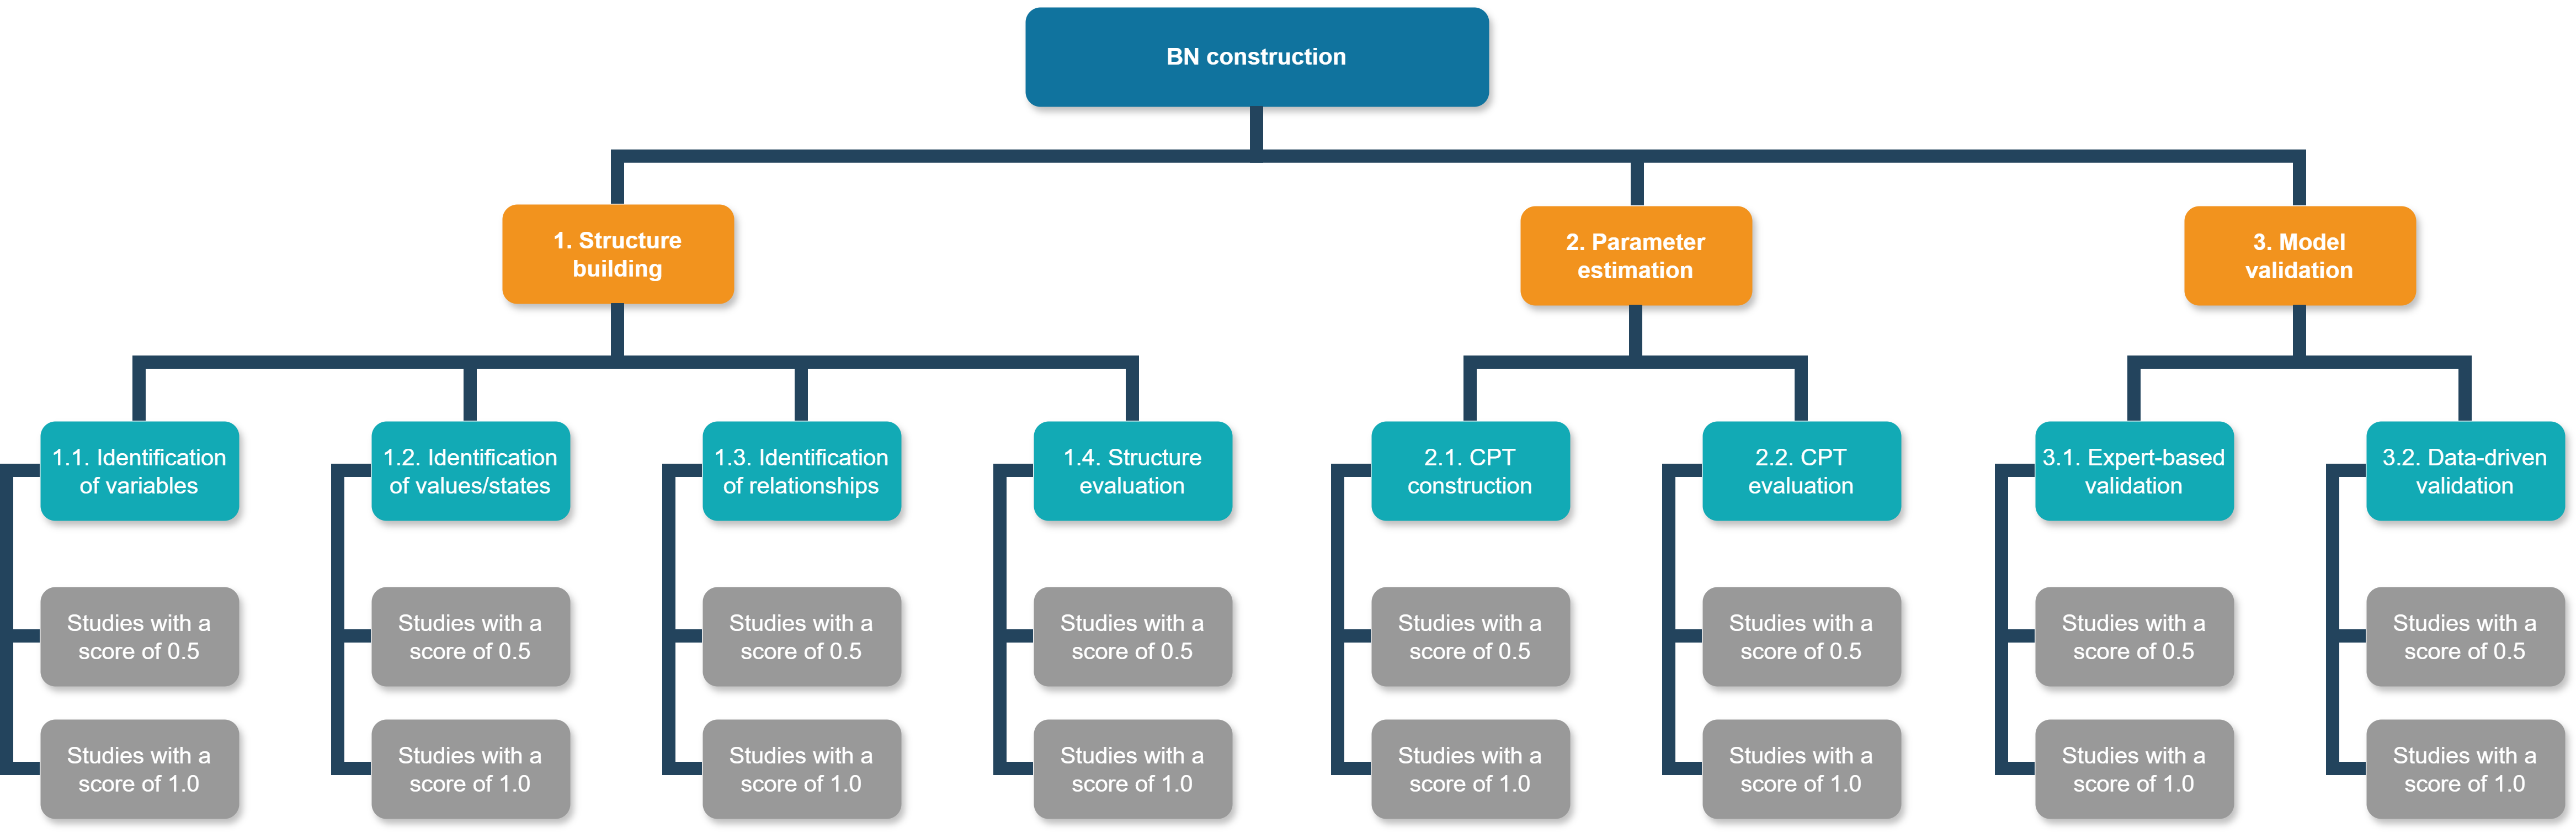
\includegraphics[width=\linewidth,angle=90]{ProtocolStructure.png}
	\end{center}
	\caption{\added[id=A]{Overview of the catalog's organization by construction phase and activity.}}
	\label{fig:protocolo_overview}
\end{figure}
\begin{table*}[t]
\caption{\added[id=A]{Checklist for assessing reported BN construction procedures}}
\label{tab:checklist_operational}
\centering
\small
\renewcommand{\arraystretch}{1.2}
\setlength{\tabcolsep}{6pt}

\begin{tabularx}{\textwidth}{>{\raggedright\arraybackslash}p{0.9cm}
                              >{\raggedright\arraybackslash}X}
\toprule
\textbf{ID} & \textbf{Assessment criterion} \\
\midrule

\multicolumn{2}{l}{\textbf{Structure building}} \\
Q1   & Is the construction of the BN structure appropriately described? \\
Q1.1 & Did the researchers detail how the model variables/factors were identified? \\ 
Q1.2 & Did the researchers detail how the node values/states were defined? \\
Q1.3 & Did the researchers detail how the relationships among the model variables/factors were identified? \\
Q1.4 & Did the researchers detail how the BN structure was evaluated? \\ 

\addlinespace[6pt]
\multicolumn{2}{l}{\textbf{Parameter estimation}} \\
Q2   & Is the estimation of the BN parameters appropriately described? \\
Q2.1 & Did the researchers detail how the CPTs were constructed? \\
Q2.2 & Did the researchers detail how the CPTs were evaluated? \\

\addlinespace[6pt]
\multicolumn{2}{l}{\textbf{Model validation}} \\
Q3   & Is the BN validation appropriately described? \\
Q3.1 & Did the researchers detail how the model was validated using an expert-driven and/or data-driven approach? \\

\bottomrule
\end{tabularx}
\end{table*}

\begin{table*}[t]
\caption{\added[id=A]{Scoring levels for the assessment of reported construction procedures}}
\label{tab:scoring_scheme}
\centering
\small
\renewcommand{\arraystretch}{1.2}
\setlength{\tabcolsep}{8pt}

\begin{tabularx}{\textwidth}{>{\centering\arraybackslash}p{1.2cm} >{\raggedright\arraybackslash}X}
\toprule
\textbf{Score} & \textbf{Interpretation} \\
\midrule
0   & No relevant information is provided, or the description is too vague to enable replication of the BN construction process. \\
0.5 & Partial information is provided, lacking sufficient detail for straightforward replication. \\
1   & The activity is clearly and comprehensively described, with sufficient detail to allow replication of the approach with minimal ambiguity. \\
\bottomrule
\end{tabularx}
\end{table*}

\added[id=A]{Given that each construction phase (structure building, parameter estimation, and model validation) contains different numbers of checklist items, we normalized their scores so that each phase contributes equally, with a maximum of one point, to the study’s total score ($S_{total}$) as follows:}

\vspace*{0.5\baselineskip}

$S_{total} = 0.25 \times Q1 + 0.5 \times Q2 + Q3$

where

$Q1 = Q1.1 + Q1.2 + Q1.3 + Q1.4$

$Q2 = Q2.1 + Q2.2$

$Q3 = Q3.1$

\vspace*{0.5\baselineskip}

\added[id=A]{To define the set of representative studies for the method catalog, we established a minimum overall score of 1.5. This threshold corresponds to the overall score obtained when all checklist items receive the intermediate score of 0.5. The selection criterion was based on the overall score rather than on a minimum score for each checklist item. Accordingly, studies with \(S_{total} \geq 1.5\) were included in this set. Studies meeting this threshold formed the evidence base for extracting methods. Inclusion identifies the studies retained under this assessment rule, not methods demonstrated to be more reliable or models demonstrated to be of higher quality.}

\begin{table*}[t]
\caption{\added[id=A]{Selected reference studies with maximum phase-level assessment scores}}
\label{tab:bons_exemplos}
\centering
\small
\renewcommand{\arraystretch}{1.15}
\setlength{\tabcolsep}{8pt}

\begin{tabularx}{\textwidth}{>{\raggedright\arraybackslash}p{45pt}
                                >{\raggedright\arraybackslash}X}
\toprule
\textbf{ID} & \textbf{Article title} \\
\midrule

\multicolumn{2}{l}{\textbf{Structure building}} \\[2pt]
PS3 & Towards improving decision making and estimating the value of decisions in value-based software engineering: the VALUE framework \\
PS4 & Using knowledge elicitation to improve Web effort estimation: Lessons from six industrial case studies \\
PS7 & Assisting the continuous improvement of Scrum projects using metrics and Bayesian networks \\

\addlinespace[6pt]
\multicolumn{2}{l}{\textbf{Parameter estimation}} \\[2pt]
PS3 & Towards improving decision making and estimating the value of decisions in value-based software engineering: the VALUE framework \\
PS7 & Assisting the continuous improvement of Scrum projects using metrics and Bayesian networks \\
PS42 & A method to estimate software strategic indicators in software development: an industrial application \\

\addlinespace[6pt]
\multicolumn{2}{l}{\textbf{Model validation}} \\[2pt]
PS3 & Towards improving decision making and estimating the value of decisions in value-based software engineering: the VALUE framework \\
PS4 & Using knowledge elicitation to improve Web effort estimation: Lessons from six industrial case studies \\
PS7 & Assisting the continuous improvement of Scrum projects using metrics and Bayesian networks \\
PS10 & Advanced Bayesian network for task effort estimation in agile software development \\
PS19 & On the effectiveness of early life cycle defect prediction with Bayesian Nets \\

\bottomrule
\end{tabularx}
\end{table*}
\FloatBarrier

\FloatBarrier

\subsection{Structure Building}

\begin{figure}[t]
  \centering
  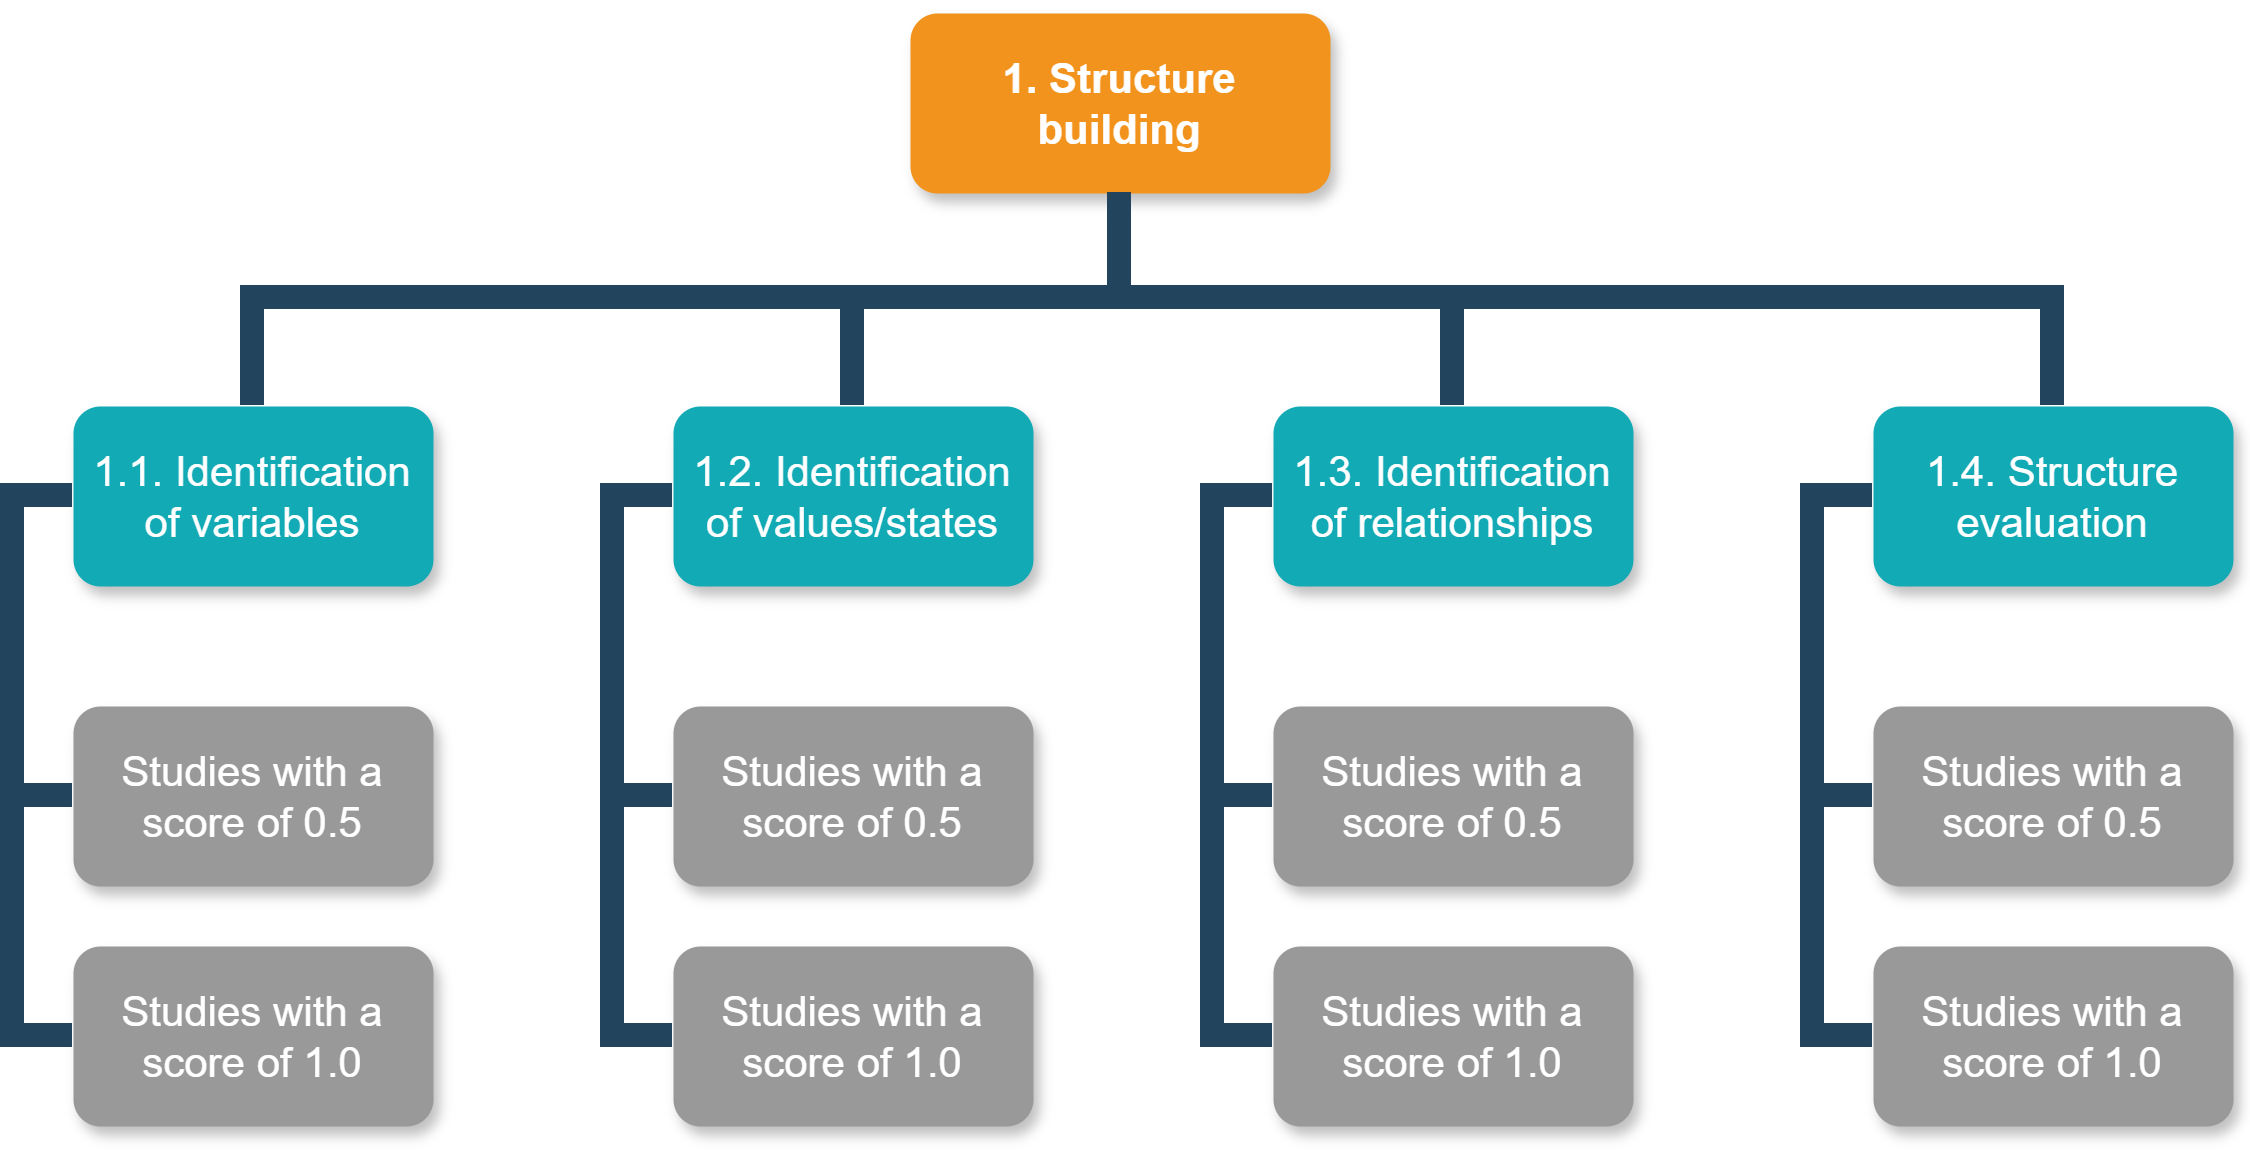
\includegraphics[width=\linewidth]{AppendixStructureBuilding.png}
  \caption{Phase 1: Structure building.}
  \Description{\added[id=A]{Diagram of the catalog's structure-building phase and its associated activities.}}
  \label{fig:app-structure-building}
\end{figure}

\begin{table}[tbp]
\caption{Studies and scores for Phase 1 (Structure building)}
\label{tab:app_phase1_scores}

\setlength{\tabcolsep}{4pt}
\begin{tabular}{p{45pt}p{45pt}p{\dimexpr\linewidth-90pt-6\tabcolsep\relax}}
\toprule
\textbf{Activity} & \textbf{Score} & \textbf{Studies} \\
\midrule

1.1 & 0.5 & PS15, PS33, PS54, PS65, PS66 \\
    & 1.0 & PS1--PS14, PS16--PS19, PS21--PS25, PS27--PS32, PS34--PS53, PS55--PS64 \\

\midrule

1.2 & 0.5 & PS11, PS13, PS17, PS19, PS21, PS24, PS29, PS39, PS47, PS48, PS52, PS56, PS61, PS62, PS66 \\
    & 1.0 & PS2--PS10, PS12, PS15, PS16, PS25, PS27, PS31, PS35, PS42, PS50, PS53, PS55, PS59, PS60, PS63--PS65 \\

\midrule

1.3 & 0.5 & PS2, PS11, PS15, PS33, PS54, PS62, PS65, PS66 \\
    & 1.0 & PS1, PS3--PS10, PS12--PS14, PS16--PS19, PS21--PS25, PS27--PS32, PS34--PS53, PS55--PS61, PS63, PS64 \\

\midrule

1.4 & 0.5 & PS24, PS52, PS59, PS61, PS66 \\
    & 1.0 & PS3--PS7, PS13, PS17, PS18, PS27, PS31, PS38, PS39, PS44, PS47, PS49, PS56, PS63 \\

\bottomrule
\end{tabular}
\end{table}

\vspace{0.5cm}

\begin{table}[t]
\caption{Methods used for structure building (variables and relationships)}
\label{tab:app_methods_var_rel}
\centering
\small
\setlength{\tabcolsep}{4pt}
\renewcommand{\arraystretch}{1.15}
\begin{tabularx}{\linewidth}{@{}>{\raggedright\arraybackslash}p{0.26\linewidth}
                            >{\raggedright\arraybackslash}X
                            >{\raggedright\arraybackslash}X@{}}
\toprule
\textbf{Method} & \textbf{1.1: Variables} & \textbf{1.3: Relationships} \\
\midrule
Interviews
& PS1, PS3, PS5, PS16, PS18, PS37, PS41, PS47, PS59, PS62
& PS1, PS8, PS16, PS18, PS41, PS47, PS59 \\
Focus groups
& PS3--PS6, PS19, PS42, PS47, PS64
& PS3--PS6, PS19, PS42, PS47 \\
Survey with practitioners
& PS57, PS58, PS64
& PS37, PS57--PS60, PS62 \\
Literature review
& PS2, PS4, PS6--PS9, PS11, PS13, PS14, PS17, PS19, PS21, PS23--PS27, PS30, PS32, PS34, PS35, PS37--PS40, PS42--PS46, PS48, PS49, PS51--PS53, PS55, PS56, PS58--PS60, PS62, PS63
& PS2, PS4, PS6, PS7, PS13, PS14, PS17, PS19, PS21, PS23--PS28, PS30, PS32, PS35, PS38--PS40, PS42--PS46, PS48, PS49, PS51--PS53, PS55, PS56, PS58 \\
Selection of variables from a dataset
& PS4, PS6, PS27, PS28
& --- \\
Delphi method
& PS7
& PS7 \\
Grounded theory
& PS3, PS5, PS41, PS57, PS58
& PS41, PS57, PS58 \\
Statistical analysis
& ---
& PS13, PS34 \\
Software analysis
& PS36
& PS36 \\
Abstraction sheets
& PS1
& PS1 \\
Idioms
& PS7, PS13, PS31, PS47, PS48, PS52
& PS7, PS13, PS31, PS47, PS48, PS52 \\
Divorcing
& ---
& PS3--PS6, PS48, PS49 \\
d-separation
& ---
& PS4, PS10, PS53 \\
Life Cycle Model (SDLC)
& PS11, PS15, PS19--PS22, PS53, PS54, PS56
& PS11, PS15, PS19--PS22, PS53, PS54, PS56 \\
Risk-centric modeling
& PS37, PS41, PS45, PS52, PS58--PS60
& PS37, PS41, PS45, PS52, PS58--PS60 \\
GQM paradigm
& PS1, PS9, PS10, PS12, PS47, PS48
& PS1, PS9, PS10, PS12, PS47, PS48 \\
Top-down approach
& PS7, PS8, PS40
& PS7, PS8, PS40 \\
Quality model
& PS33, PS42, PS50
& PS33, PS42, PS50 \\
Value model
& PS3
& PS3 \\
Argumentation model
& PS29
& PS29 \\
K2 algorithm
& PS61
& PS61, PS64 \\
NPC algorithm
& PS63
& PS63 \\
Cheng's algorithm
& ---
& PS59, PS60 \\
V-structure discovery algorithm
& ---
& PS60 \\
Learning from data using an automated tool
& PS65, PS66
& PS3, PS62, PS65, PS66 \\
\bottomrule
\end{tabularx}
\end{table}

\begin{table}[t]
\caption{Methods used to define node states (Activity 1.2)}
\label{tab:app_methods_node_states}
\centering
\small
\setlength{\tabcolsep}{4pt}
\renewcommand{\arraystretch}{1.15}
\begin{tabularx}{\linewidth}{@{}>{\raggedright\arraybackslash}p{0.38\linewidth}
                            >{\raggedright\arraybackslash}X@{}}
\toprule
\textbf{Method} & \textbf{Studies (Activity 1.2)} \\
\midrule
Expert-derived categories/thresholds
& PS1--PS17, PS19, PS21, PS23--PS25, PS27--PS29, PS31, PS36, PS39, PS41, PS42, PS44, PS47, PS50, PS52--PS56, PS59, PS61, PS66 \\
Automatic discretization
& PS1, PS12, PS27, PS35, PS42, PS48, PS55, PS57, PS61--PS66 \\
Literature review
& PS40, PS43, PS60 \\
\bottomrule
\end{tabularx}
\end{table}

\begin{table}[t]
\caption{Methods used to evaluate the structure (Activity 1.4)}
\label{tab:app_methods_structure_evaluation}
\centering
\small
\setlength{\tabcolsep}{4pt}
\renewcommand{\arraystretch}{1.15}
\begin{tabularx}{\linewidth}{@{}>{\raggedright\arraybackslash}p{0.38\linewidth}
                            >{\raggedright\arraybackslash}X@{}}
\toprule
\textbf{Method} & \textbf{Studies (Activity 1.4)} \\
\midrule
Interviews & PS49 \\
Focus groups & PS3--PS6 \\
Survey with practitioners & PS38, PS39, PS44, PS56 \\
Statistical analysis & PS27, PS38, PS44, PS63 \\
Simulated association rules & PS17 \\
Expert review & PS7, PS13, PS18, PS24, PS31, PS47, PS52, PS59, PS61, PS63 \\
\bottomrule
\end{tabularx}
\end{table}

\subsubsection{Reference Studies for Structure Building}

The following studies were identified as reference studies for the structure building phase, as they achieved a score of 1.0 in all activities (Activities 1.1--1.4):

\begin{itemize}
    \item Mendes, E., Rodriguez, P., Freitas, V., Baker, S., \& Atoui, M. A. (2018). Towards improving decision making and estimating the value of decisions in value-based software engineering: The VALUE framework. \textit{Software Quality Journal}, 26(2), 607--656. [PS3]
    
    \item Mendes, E. (2012). Using knowledge elicitation to improve web effort estimation: Lessons from six industrial case studies. In \textit{Proceedings of the 34th International Conference on Software Engineering (ICSE)} (pp. 1112--1121). IEEE. [PS4]
    
    \item Mendes, E., Vaz, V. T., \& Muradas, F. (2015). An expert-based requirements effort estimation model using Bayesian networks. In \textit{International Conference on Software Quality} (pp. 79--93). Springer. [PS5]
    
    \item Mendes, E. (2013). Using expert-based Bayesian networks as decision support systems to improve project management of healthcare software projects. In \textit{International Conference on Software Engineering and Applications} (Vol. 2, pp. 389--399). SCITEPRESS. [PS6]
    
    \item Perkusich, M., Gorgônio, K. C., Almeida, H., \& Perkusich, A. (2017). Assisting the continuous improvement of Scrum projects using metrics and Bayesian networks. \textit{Journal of Software: Evolution and Process}, 29(6), e1835. [PS7]
    
    \item Pendharkar, P. C., Subramanian, G. H., \& Rodger, J. A. (2005). A probabilistic model for predicting software development effort. \textit{IEEE Transactions on Software Engineering}, 31(7), 615--624. [PS27]
    
    \item Perkusich, M., Medeiros, A., e Silva, L. C., Gorgônio, K. C., de Almeida, H. O., \& Perkusich, A. (2015). A Bayesian network approach to assist on the interpretation of software metrics. In \textit{Proceedings of the 30th Annual ACM Symposium on Applied Computing} (pp. 1498--1503). [PS31]
    
    \item Mendes, E. (2007). The use of a Bayesian network for web effort estimation. In \textit{International Conference on Web Engineering} (pp. 90--104). Springer. [PS63]
\end{itemize}

\added[id=A]{These studies provide reference examples of reported variable identification, state definition, relationship elicitation, and structure evaluation. Their selection reflects the phase-level assessment scores rather than an independent comparison of the quality of their BN models.}

\subsection{Parameter Estimation}

\begin{figure}[t]
  \centering
  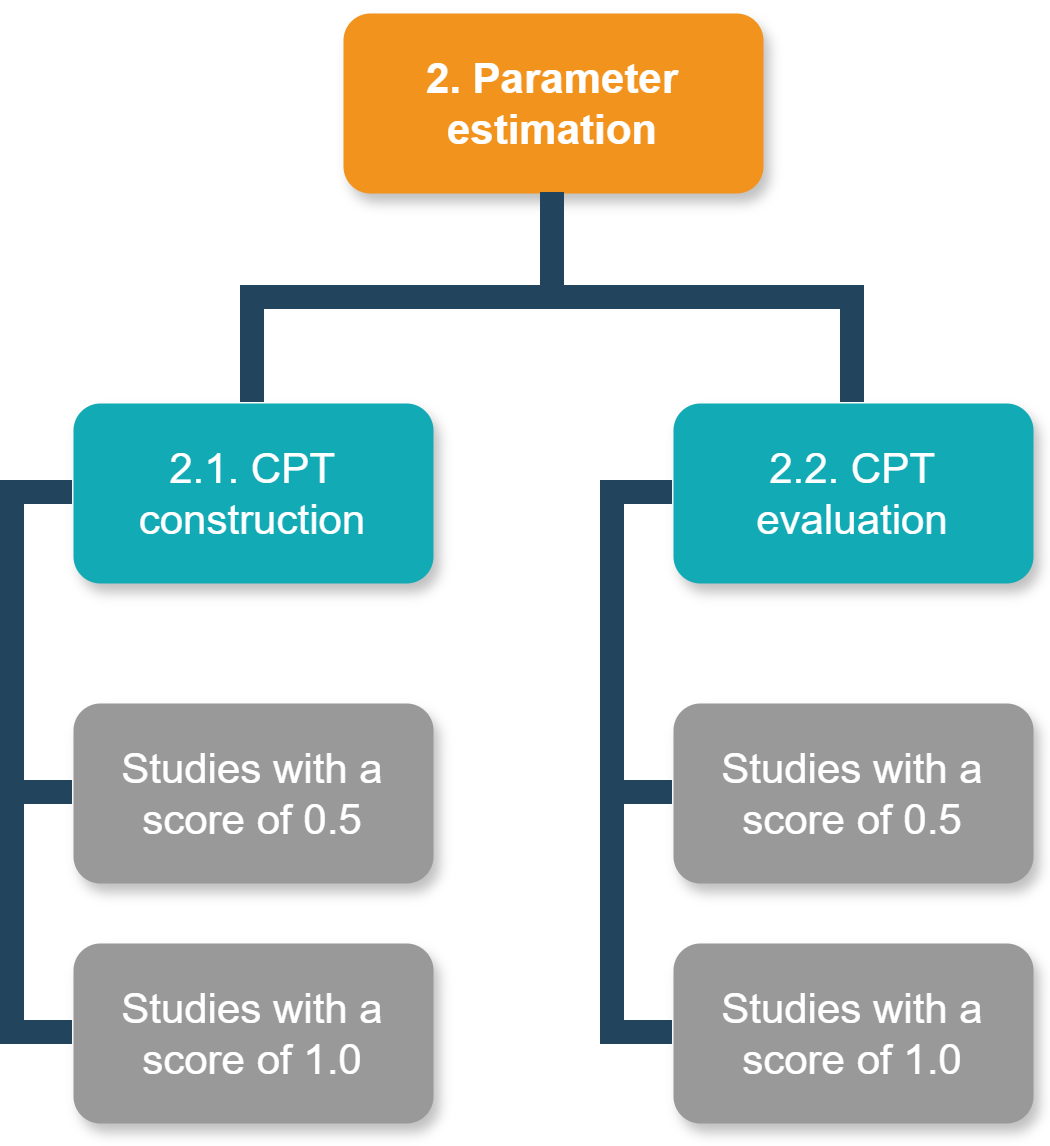
\includegraphics[width=\linewidth,height=0.42\textheight,keepaspectratio]{AppendixParameterEstimation.png}
  \caption{Phase 2: Parameter estimation.}
  \Description{\added[id=A]{Diagram of the catalog's parameter-estimation phase and its associated activities.}}
  \label{fig:app-estimativa-parametros}
\end{figure}

\begin{table}[t]
\caption{Studies and scores for Phase 2 (Parameter estimation)}
\label{tab:app_phase2_scores}
\centering
\small
\setlength{\tabcolsep}{4pt}
\renewcommand{\arraystretch}{1.15}
\begin{tabular}{p{45pt}p{45pt}p{\dimexpr\linewidth-90pt-6\tabcolsep\relax}}
\toprule
\textbf{Activity} & \textbf{Score} & \textbf{Studies} \\
\midrule

2.1 & 0.5 & PS9, PS12, PS17, PS21, PS35, PS36, PS39, PS40, PS46, PS50, PS52, PS56, PS63 \\
    & 1.0 & PS1--PS3, PS7, PS8, PS13, PS14, PS19, PS20, PS22--PS26, PS29, PS31, PS33, PS34, PS37, PS38, PS42, PS44, PS47, PS48, PS53, PS54, PS58 \\

\midrule

2.2 & 0.5 & PS2, PS12, PS20, PS21, PS33, PS47, PS63 \\
    & 1.0 & PS3, PS7, PS17, PS42 \\

\bottomrule
\end{tabular}
\end{table}

\begin{table}[t]
\caption{Methods used for CPT construction (Activity 2.1)}
\label{tab:app_methods_cpt_construction}
\centering
\small
\setlength{\tabcolsep}{4pt}
\renewcommand{\arraystretch}{1.15}
\begin{tabularx}{\linewidth}{@{}>{\raggedright\arraybackslash}p{0.40\linewidth}
                            >{\raggedright\arraybackslash}X@{}}
\toprule
\textbf{Method} & \textbf{Studies (Activity 2.1)} \\
\midrule
Interviews & PS8, PS13, PS49 \\
Focus groups & PS3--PS6, PS48 \\
Literature review & PS17, PS21, PS22, PS35, PS48, PS56 \\
Survey with practitioners & PS9, PS13, PS18, PS25, PS31, PS37--PS39, PS43, PS44, PS47, PS56--PS60 \\
Analytic Hierarchy Process (AHP) & PS26 \\
Theoretical modeling & PS29 \\
Frequency quantification from historical/empirical data & PS2, PS3, PS20, PS24, PS30, PS38, PS42, PS44, PS48, PS52 \\
Frequency estimation from simulated data & PS46 \\
Noisy-OR gates & PS33, PS36, PS50 \\
Direct functions & PS2, PS21, PS29, PS34, PS36, PS39, PS50, PS51, PS53 \\
Expert-derived functions & PS48 \\
Ranked nodes method & PS1, PS7--PS9, PS12, PS19, PS22, PS23, PS31, PS40, PS43, PS47, PS53 \\
Partitioned expressions & PS12, PS19, PS47 \\
Weighted Sum Algorithm (WSA) & PS3, PS4, PS42 \\
Distribution fitting & PS13, PS21, PS22, PS26, PS29, PS33 \\
Probability extrapolation & PS20 \\
Parametric learning & PS14 \\
Fuzzy logic & PS35, PS48, PS54 \\
Quantifying Judgment (QJ) method & PS24, PS25 \\
Generalized Linear Model (GLM) & PS34, PS51 \\
Expectation-Maximization (EM) algorithm & PS36, PS37, PS58, PS63 \\
Maximum Likelihood Estimation (MLE) & PS34 \\
Learning from data using an automated tool & PS10, PS12, PS15, PS16, PS18, PS28, PS44, PS55, PS65, PS66 \\
\bottomrule
\end{tabularx}
\end{table}

\begin{table}[t]
\caption{Methods used for CPT evaluation (Activity 2.2)}
\label{tab:app_methods_cpt_evaluation}
\centering
\small
\setlength{\tabcolsep}{4pt}
\renewcommand{\arraystretch}{1.15}
\begin{tabularx}{\linewidth}{@{}>{\raggedright\arraybackslash}p{0.42\linewidth}
                            >{\raggedright\arraybackslash}X@{}}
\toprule
\textbf{Method} & \textbf{Studies (Activity 2.2)} \\
\midrule
Expert review & PS2, PS12, PS20, PS21, PS28, PS33, PS41, PS42, PS47, PS63 \\
Focus groups & PS3, PS5, PS6 \\
Brier score & PS7 \\
Simulated relevance analysis & PS17 \\
\bottomrule
\end{tabularx}
\end{table}

\subsubsection{Reference Studies for Parameter Estimation}

The following studies were identified as reference studies for the parameter estimation phase, as they achieved a score of 1.0 in all activities (Activities 2.1--2.2):

\begin{itemize}
    \item Mendes, E., Rodriguez, P., Freitas, V., Baker, S., \& Atoui, M. A. (2018). Towards improving decision making and estimating the value of decisions in value-based software engineering: The VALUE framework. \textit{Software Quality Journal}, 26(2), 607--656. [PS3]
    
    \item Perkusich, M., Gorgônio, K. C., Almeida, H., \& Perkusich, A. (2017). Assisting the continuous improvement of Scrum projects using metrics and Bayesian networks. \textit{Journal of Software: Evolution and Process}, 29(6), e1835. [PS7]
    
    \item Manzano, M., Ayala, C., Gómez, C., Abherve, A., Franch, X., \& Mendes, E. (2021). A method to estimate software strategic indicators in software development: An industrial application. \textit{Information and Software Technology}, 129, 106433. [PS42]
\end{itemize}

\added[id=A]{These studies provide reference examples of reported CPT construction and evaluation procedures. Their selection reflects the phase-level assessment scores rather than demonstrated superiority of their methods or models.}

\subsection{Model Validation}

\begin{figure}[t]
  \centering
  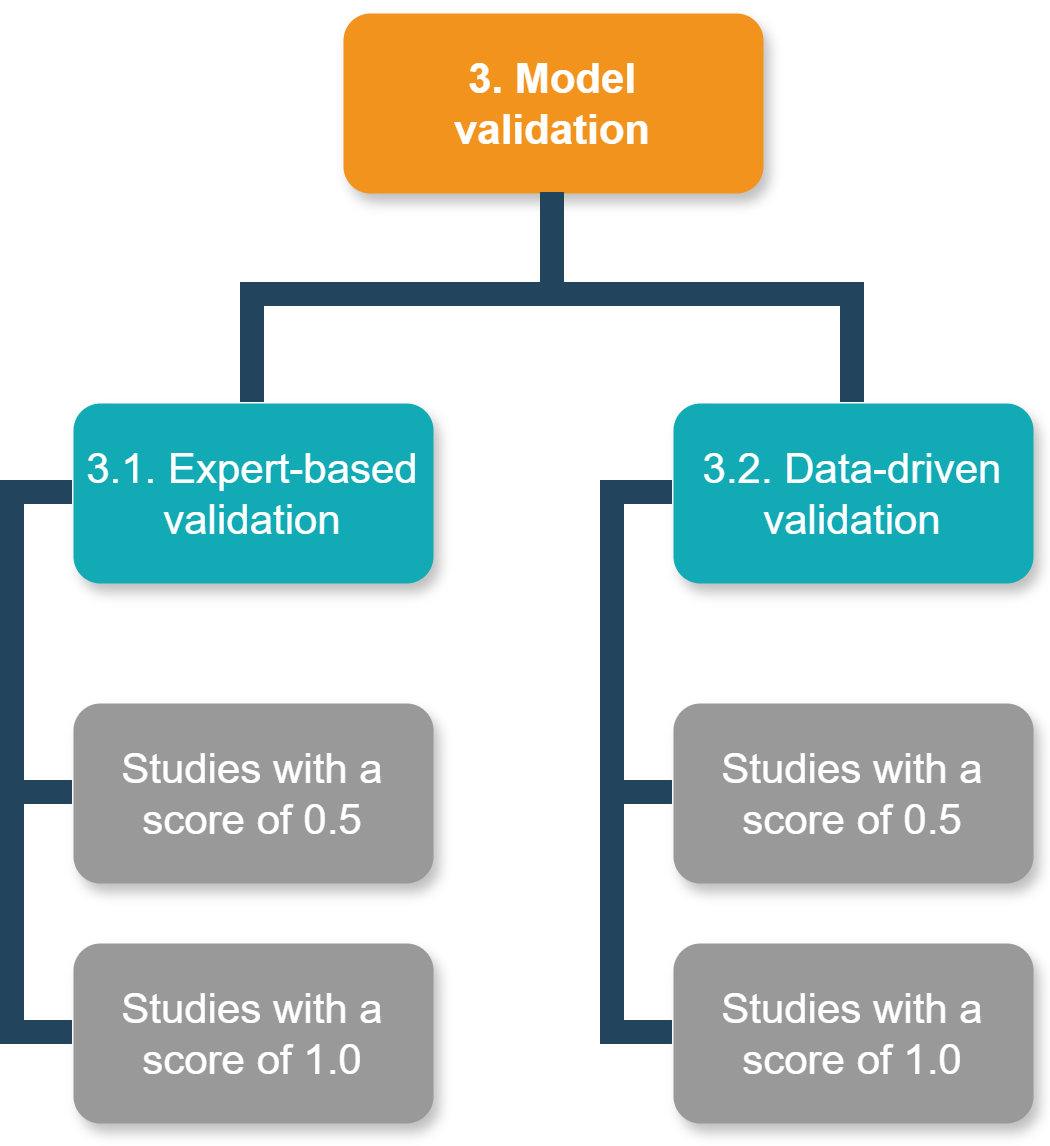
\includegraphics[width=\linewidth,height=0.42\textheight,keepaspectratio]{AppendixModelValidation.png}
  \caption{Phase 3: Model validation.}
  \Description{\added[id=A]{Diagram of the catalog's model-validation phase and its associated activities.}}
  \label{fig:app-validacao-modelo}
\end{figure}

\begin{table}[t]
\caption{Studies and scores for Phase 3 (Model validation - Activities 3.1 and 3.2)}
\label{tab:app_phase3_scores}
\centering
\small
\setlength{\tabcolsep}{4pt}
\renewcommand{\arraystretch}{1.15}
\begin{tabular}{p{55pt}p{55pt}p{\dimexpr\linewidth-110pt-6\tabcolsep\relax}}
\toprule
\textbf{Activity} & \textbf{Score} & \textbf{Studies} \\
\midrule

3.1/3.2 & 0.5 & PS2, PS21, PS23, PS24, PS29, PS33, PS35, PS37, PS50, PS52, PS56 \\
        & 1.0 & PS1, PS3--PS16, PS18--PS20, PS22, PS25--PS28, PS30--PS32, PS34, PS36, PS38--PS49, PS51, PS53--PS55, PS57--PS66 \\

\bottomrule
\end{tabular}
\end{table}

\begin{table}[t]
\caption{Methods used for model validation (Activities 3.1 and 3.2)}
\label{tab:app_methods_model_validation}
\centering
\small
\setlength{\tabcolsep}{4pt}
\renewcommand{\arraystretch}{1.15}
\begin{tabularx}{\linewidth}{@{}>{\raggedright\arraybackslash}p{0.42\linewidth}
                            >{\raggedright\arraybackslash}X@{}}
\toprule
\textbf{Method} & \textbf{Studies (Activities 3.1/3.2)} \\
\midrule
Model walkthrough
& PS1, PS3, PS4, PS6, PS7, PS9, PS12, PS14, PS20, PS32, PS40--PS43, PS47, PS49, PS52 \\

Sensitivity analysis
& PS2, PS12, PS19, PS26, PS44 \\

Focus groups
& PS41 \\

Case study
& PS8, PS25, PS31, PS46, PS53, PS57, PS58 \\

Proof of concept
& PS2, PS19, PS21, PS23, PS24, PS29, PS33, PS35, PS37, PS50, PS56 \\

Predictive accuracy
& PS3--PS6, PS8, PS18--PS20, PS28, PS31, PS36, PS42, PS45, PS63, PS64 \\

Cross-validation
& PS10, PS15, PS16, PS30, PS38, PS57, PS59, PS60, PS65 \\

Statistical measures
& PS10, PS11, PS13--PS16, PS19, PS22, PS32, PS34, PS36, PS39, PS44, PS48, PS51, PS54, PS55, PS57, PS59, PS61--PS63, PS66 \\

Comparison with existing models
& PS27, PS34, PS44, PS51, PS54, PS59, PS60 \\

\bottomrule
\end{tabularx}
\end{table}

\subsubsection{Reference Studies for Model Validation}

The following studies were identified as reference studies for the model validation phase, as they achieved a score of 1.0 in at least one of the validation activities (Activity 3.1 or 3.2):

\small
\begin{itemize}

\item Saraiva, R. M., Perkusich, M. B., Almeida, H. O., \& Perkusich, A. (2017).
A process to calculate the uncertainty of software metrics-based models using Bayesian networks.
In \textit{SEKE} (pp. 467--472). [PS1]

\item Mendes, E., Rodriguez, P., Freitas, V., Baker, S., \& Atoui, M. A. (2018).
Towards improving decision making and estimating the value of decisions in value-based software engineering: The VALUE framework.
\textit{Software Quality Journal}, 26(2), 607--656. [PS3]

\item Mendes, E. (2012).
Using knowledge elicitation to improve web effort estimation: Lessons from six industrial case studies.
In \textit{2012 34th International Conference on Software Engineering (ICSE)} (pp. 1112--1121). IEEE. [PS4]

\item Mendes, E., Vaz, V. T., \& Muradas, F. (2015).
An expert-based requirements effort estimation model using Bayesian networks.
In \textit{International Conference on Software Quality} (pp. 79--93). Springer. [PS5]

\item Mendes, E. (2013).
Using expert-based Bayesian networks as decision support systems to improve project management of healthcare software projects.
In \textit{International Conference on Software Engineering and Applications} (Vol. 2, pp. 389--399). SCITEPRESS. [PS6]

\item Perkusich, M., Gorgônio, K. C., Almeida, H., \& Perkusich, A. (2017).
Assisting the continuous improvement of Scrum projects using metrics and Bayesian networks.
\textit{Journal of Software: Evolution and Process}, 29(6), e1835. [PS7]

\item Freire, A., Perkusich, M., Saraiva, R., Almeida, H., \& Perkusich, A. (2018).
A Bayesian networks-based approach to assess and improve the teamwork quality of agile teams.
\textit{Information and Software Technology}, 100, 119--132. [PS8]

\item Willamy, R., Nunes, J., Perkusich, M. B., Freire, A. S., Saraiva, R. M., Almeida, H. O., \& Perkusich, A. (2016).
A method to build Bayesian networks based on artifacts and metrics to assess agile projects.
In \textit{SEKE} (pp. 81--86). [PS9]

\item Turic, M., Celar, S., Dragicevic, S., \& Vickovic, L. (2023).
Advanced Bayesian network for task effort estimation in agile software development.
\textit{Applied Sciences}, 13(16), 9465. [PS10]

\item Kumar, C., \& Yadav, D. K. (2017).
Software defects estimation using metrics of early phases of software development life cycle.
\textit{International Journal of System Assurance Engineering and Management}, 8(Suppl 4), 2109--2117. [PS11]

\item Schulz, T., Radliński, Ł., Gorges, T., \& Rosenstiel, W. (2013).
Predicting the flow of defect correction effort using a Bayesian network model.
\textit{Empirical Software Engineering}, 18(3), 435--477. [PS12]

\item Misirli, A. T., \& Bener, A. B. (2014).
Bayesian networks for evidence-based decision-making in software engineering.
\textit{IEEE Transactions on Software Engineering}, 40(6), 533--554. [PS13]

\item Berdún, L., Pace, J. A. D., Amandi, A., \& Campo, M. (2008).
Assisting novice software designers by an expert designer agent.
\textit{Expert Systems with Applications}, 34(4), 2772--2782. [PS14]

\item Amasaki, S., Takagi, Y., Mizuno, O., \& Kikuno, T. (2005).
Constructing a Bayesian belief network to predict final quality in embedded system development.
\textit{IEICE Transactions on Information and Systems}, 88(6), 1134--1141. [PS15]

\item Song, T. H., Yoon, K. A., \& Bae, D. H. (2007).
An approach to probabilistic effort estimation for military avionics software maintenance by considering structural characteristics.
In \textit{14th Asia-Pacific Software Engineering Conference (APSEC'07)} (pp. 406--413). IEEE. [PS16]

\item Pérez-Miñana, E., \& Gras, J. J. (2006).
Improving fault prediction using Bayesian networks for the development of embedded software applications.
\textit{Software Testing, Verification and Reliability}, 16(3), 157--174. [PS18]

\item Fenton, N., Neil, M., Marsh, W., Hearty, P., Radliński, Ł., \& Krause, P. (2008).
On the effectiveness of early life cycle defect prediction with Bayesian Nets.
\textit{Empirical Software Engineering}, 13(5), 499--537. [PS19]

\item Fenton, N., Krause, P., \& Neil, M. (2002).
Probabilistic modelling for software quality control.
\textit{Journal of Applied Non-Classical Logics}, 12(2), 173--188. [PS20]

\item Hearty, P., Fenton, N., Marquez, D., \& Neil, M. (2008).
Predicting project velocity in XP using a learning dynamic Bayesian network model.
\textit{IEEE Transactions on Software Engineering}, 35(1), 124--137. [PS22]

\item Donohue, S. K., Dugan, J. B., \& Brown, C. L. (2005).
Is my software ``good enough'' to release? A probabilistic assessment.
In \textit{IEEE/NASA Software Engineering Workshop} (pp. 5--13). IEEE. [PS25]

\item Wu, Y. P., Hu, Q. P., Poh, K. L., Ng, S. H., \& Xie, M. (2005).
Bayesian networks modeling for software inspection effectiveness.
In \textit{11th Pacific Rim International Symposium on Dependable Computing (PRDC'05)} (pp. 7). IEEE. [PS26]

\item Pendharkar, P. C., Subramanian, G. H., \& Rodger, J. A. (2005).
A probabilistic model for predicting software development effort.
\textit{IEEE Transactions on Software Engineering}, 31(7), 615--624. [PS27]

\item Stamelos, I., Angelis, L., Dimou, P., \& Sakellaris, E. (2003).
On the use of Bayesian belief networks for the prediction of software productivity.
\textit{Information and Software Technology}, 45(1), 51--60. [PS28]

\item Beaver, J. M., Schiavone, G. A., \& Berrios, J. S. (2005).
Predicting software suitability using a Bayesian belief network.
In \textit{Fourth International Conference on Machine Learning and Applications (ICMLA'05)} (pp. 7). IEEE. [PS30]

\item Perkusich, M., Medeiros, A., e Silva, L. C., Gorgônio, K. C., de Almeida, H. O., \& Perkusich, A. (2015).
A Bayesian network approach to assist on the interpretation of software metrics.
In \textit{Proceedings of the 30th Annual ACM Symposium on Applied Computing} (pp. 1498--1503). [PS31]

\item Torkar, R., Awan, N. M., Alvi, A. K., \& Afzal, W. (2010).
Predicting software test effort in iterative development using a dynamic Bayesian network.
In \textit{21st IEEE International Symposium on Software Reliability Engineering}. IEEE. [PS32]

\item Mohanta, S., Vinod, G., \& Mall, R. (2011).
A technique for early prediction of software reliability based on design metrics.
\textit{International Journal of System Assurance Engineering and Management}, 2(4), 261--281. [PS34]

\item Mirarab, S., Hassouna, A., \& Tahvildari, L. (2007).
Using Bayesian belief networks to predict change propagation in software systems.
In \textit{15th IEEE International Conference on Program Comprehension (ICPC'07)} (pp. 177--188). IEEE. [PS36]

\item Procaccino, J. D., Verner, J. M., Darter, M. E., \& Amadio, W. J. (2005).
Toward predicting software development success from the perspective of practitioners: An exploratory Bayesian model.
\textit{Journal of Information Technology}, 20(3), 187--200. [PS38]

\item Durán, M., Juárez-Ramírez, R., Jiménez, S., \& Tona, C. (2020).
User story estimation based on the complexity decomposition using Bayesian networks.
\textit{Programming and Computer Software}, 46(8), 569--583. [PS39]

\item Radu, L. D. (2019).
Effort prediction in agile software development with Bayesian networks.
In \textit{ICSOFT} (pp. 238--245). [PS40]

\item Dantas, E., Neto, A. S., Perkusich, M., Almeida, H., \& Perkusich, A. (2021).
Using Bayesian networks to support managing technological risk on software projects.
In \textit{ISE (Brazilian Workshop on Intelligent Software Engineering)} (pp. 1--6). SBC. [PS41]

\item Manzano, M., Ayala, C., Gómez, C., Abherve, A., Franch, X., \& Mendes, E. (2021).
A method to estimate software strategic indicators in software development: An industrial application.
\textit{Information and Software Technology}, 129, 106433. [PS42]

\item Handhika, T., Sutanto, Y., Juarna, A., \& Mutiara, A. B. (2021).
Bayesian analysis in predicting the success rate of the Scrum-based software development project under stochastic environment. [PS43]

\item Fatima, R., Zeshan, F., Ahmad, A., Hamid, M., Filali, I., Alhussan, A. A., \& Abdallah, H. A. (2023).
Requirement change prediction model for small software systems.
\textit{Computers}, 12(8), 164. [PS44]

\item Nguyen, N. T., Huynh, Q. T., \& Vu, T. H. G. (2018).
A Bayesian critical path method for managing common risks in software project scheduling.
In \textit{International Symposium on Information and Communication Technology} (pp. 382--388). [PS45]

\item Salama, M., \& Bahsoon, R. (2017).
Analysing and modelling runtime architectural stability for self-adaptive software.
\textit{Journal of Systems and Software}, 133, 95--112. [PS46]

\item Saraiva, R., Medeiros, A., Perkusich, M., Valadares, D., Gorgonio, K. C., Perkusich, A., \& Almeida, H. (2020).
A Bayesian networks-based method to analyze the validity of the data of software measurement programs.
\textit{IEEE Access}, 8, 198801--198821. [PS47]

\item Malak, G., Sahraoui, H., Badri, L., \& Badri, M. (2010).
Modeling web quality using a probabilistic approach: An empirical validation.
\textit{ACM Transactions on the Web (TWEB)}, 4(3), 1--31. [PS48]

\item Lamersdorf, A., \& Münch, J. (2010).
A multi-criteria distribution model for global software development projects.
\textit{Journal of the Brazilian Computer Society}, 16(2), 97--115. [PS49]

\item Khanna, M., Chauhan, N., Sharma, D. K., \& Toofani, A. (2017).
Test case prioritisation during web application testing.
\textit{International Journal of Computer Applications in Technology}, 56(3), 230--243. [PS51]

\item Eom, H. S., Park, G. Y., Jang, S. C., Son, H. S., \& Kang, H. G. (2013).
V\&V-based remaining fault estimation model for safety--critical software of a nuclear power plant.
\textit{Annals of Nuclear Energy}, 51, 38--49. [PS53]

\item Chatterjee, S., \& Maji, B. (2018).
A Bayesian belief network based model for predicting software faults in early phase of software development process.
\textit{Applied Intelligence}, 48(8), 2214--2228. [PS54]

\item Chatzimparmpas, A., \& Bibi, S. (2019).
Maintenance process modeling and dynamic estimations based on Bayesian networks and association rules.
\textit{Journal of Software: Evolution and Process}, 31(9), e2163. [PS55]

\item Wiesweg, F., Vogelsang, A., \& Mendez, D. (2020).
Data-driven risk management for requirements engineering: An automated approach based on Bayesian networks.
In \textit{IEEE Requirements Engineering Conference (RE)} (pp. 125--135). IEEE. [PS57]

\item Kalinowski, M., Curty, P., Paes, A., Ferreira, A., Spínola, R., Fernández, D. M., \ldots\ \& Wagner, S. (2017).
Supporting defect causal analysis in practice with cross-company data on causes of requirements engineering problems.
In \textit{2017 IEEE/ACM 39th International Conference on Software Engineering: Software Engineering in Practice Track (ICSE-SEIP)} (pp. 223--232). IEEE. [PS58]

\item Hu, Y., Mo, X., Zhang, X., Zeng, Y., Du, J., \& Xie, K. (2012).
Intelligent analysis model for outsourced software project risk using constraint-based Bayesian network.
\textit{J. Softw.}, 7(2), 440--449. [PS59]

\item Hu, Y., Zhang, X., Ngai, E. W. T., Cai, R., \& Liu, M. (2013).
Software project risk analysis using Bayesian networks with causality constraints.
\textit{Decision Support Systems}, 56, 439--449. [PS60]

\item Bibi, S., Stamelos, I., \& Angelis, L. (2003).
Bayesian belief networks as a software productivity estimation tool.
In \textit{Balkan Conference in Informatics} (Thessaloniki, Greece). [PS61]

\item Hamdan, K., Bibi, S., Angelis, L., \& Stamelos, I. (2009).
A Bayesian belief network cost estimation model that incorporates cultural and project leadership factors.
In \textit{IEEE Symposium on Industrial Electronics \& Applications} (Vol. 2, pp. 985--989). IEEE. [PS62]

\item Mendes, E. (2007).
The use of a Bayesian network for web effort estimation.
In \textit{International Conference on Web Engineering} (pp. 90--104). Springer. [PS63]

\item Wang, X., Wu, C., \& Ma, L. (2010).
Software project schedule variance prediction using Bayesian network.
In \textit{2010 IEEE International Conference on Advanced Management Science (ICAMS 2010)} (Vol. 2, pp. 26--30). IEEE. [PS64]

\item Pendharkar, P. C., \& Rodger, J. A. (2010).
Probabilistic and analytical estimation of software development team size.
\textit{International Journal of Hybrid Intelligent Systems}, 7(2), 137--153. [PS65]

\item Fuentetaja, R., Borrajo, D., López, C. L., \& Ocón, J. (2013).
Multi-step generation of Bayesian networks models for software projects estimations.
\textit{International Journal of Computational Intelligence Systems}, 6(5), 796--821. [PS66]

\end{itemize}
\normalsize

\FloatBarrier
\bibliographystyle{plainnat}
\bibliography{supplement-references}
\end{document}
